%\documentclass[12pt,letterpaper,doublespaced,ETD,dvips,proposal]{gt-ece-thesis}
\documentclass[12pt,letterpaper,doublespaced,ETD,proposal]{gt-ece-thesis}

\title{Multi-Target Tracking Using Residual Vector Quantization}
\author{Salman Aslam}
\copyrightyear{2010}
\graddate{December 2010}  
\approvaldate{July 2004}  

\addadvisor{Dr. Christopher F. Barnes}{Asst. Professor, School of ECE}{Georgia Institute of Technology}
\addchair{Dr. Aaron Bobick}{Professor, CoC}{Georgia Institute of Technology}
\addreader{Dr. Wayne Geronimo}{Asst. Professor, School of ECE}{Georgia Institute of Technology}
\addreader{Dr. David Goliath}{Asst. Professor, School of ECE}{Georgia Institute of Technology}
\addreader{Dr. Marky Mark}{Asst. Professor, School of ECE}{Georgia Institute of Technology}
\addreader{Dr. Larry A. Stooge}{Asst. Professor, School of ECE}{Georgia Institute of Technology}


\bibfiles{c:/salman/work/writing/MyCitations}

\titlepagetrue
\figurespagetrue
\tablespagetrue
\contentspagetrue
\symbolspagefalse
\glossarypagefalse 
\bibpagetrue
\mastersthesisfalse 
\multivolumefalse
\singlespacednotestrue

\usepackage{graphicx, subfigure}
\usepackage{insfig}
\usepackage{url}
\usepackage{multirow}
\usepackage{hyperref}

\setchaptertocdepth{2}
\setappendixtocdepth{2}

\settocstring{Table of Contents}
\setlofstring{List of Figures}
%\setlotstring{List of Tables}
\setbibstring{References}
\setindstring{Index}
\setdedstring{Dedication}
\setglostring{List of Terms}
\setchpstring{Chapter}
\setappstring{Appendix}
\setprtstring{Volume}
\setabsstring{Summary}
\setlosstring{List of Symbols}
\setackstring{Acknowledgment}

\setfrontpagestyle{plain}
\setbodypagestyle{plain}
\setendpagestyle{plain}


\begin{document}
	
	\pagestyle{plain}
	\bibliographystyle{ieeetr}

	\begin{FrontMatter}
		\contents %Generates the TOC, LOF, and LOT
	\end{FrontMatter}

	\begin{Body}	
		
%------------------------------------------------------------------------------
\section{Introduction}
\label{intro}	
%------------------------------------------------------------------------------
 \par
Images have fascinated humans for thousands of years.  The earliest cave paintings have been dated back to around 30,000 years \cite{2009_WEB_EarliestHumanPaintings_Gray}.  Currently, several fields deal with the creation and analysis of images.  Some example fields are art, photography, calligraphy and digital forensics.  In this work, we are primarily interested in the computational processing of images.  The three primary fields dealing with this aspect of images are Image Processing, Computer Vision and Computer Graphics.  The field of Image Processing deals with low level image analysis, Computer Vision deals with high level image analysis, and Computer Graphics primarily deals with image synthesis.  Within the field of Computer Vision, we are interested in tracking multiple objects in image sequences.

Object tracking, target tracking, or simply tracking, can be defined as estimating the trajectory of an object of interest over time.  In practical applications, tracking is normally preceded by a detection step and succeeded by a track analysis step \cite{2006_JNL_SURVEYtrk_Yilmaz}:

\begin{itemize}
\item \textbf{Detection}.  In this step, objects of interest are identified and segmented.  A background model is commonly used as a pre-processing step.
\item  \textbf{Tracking}.  The detected objects of interest are tracked from frame to frame.  
\item  \textbf{Track analysis}.  In this step, track information is fused to infer higher semantic knowledge.
\end{itemize}

Recently, there has been a surge in interest in tracking due to several reasons: (a) proliferation of powerful computers, (b) availability of high quality and inexpensive video cameras, and (c) an increasing need for automated video analysis.  However, many practical difficulties are encountered during multi-target visual-tracking:

\begin{itemize}
\item Loss of information caused by projecting 3D world objects onto 2D images
\item Sudden illumination changes
\item Appearance drifts
\item Complex target motion, including acceleration
\item Non-rigid or articulated nature of objects
\item Object-to-object merges/splits/occlusions
\item Object-to-scene occlusions
\item Camera motion
\item Noise
\item Real time processing requirements
\end{itemize} 

Clearly, visual tracking is a challenging problem.  Under general conditions, it remains an unsolved problem.  Several researchers have tried to approach this problem by specifying additional constraints on the targets being tracked.  Constraints have also been placed on the tracking environment.  For example, almost all tracking algorithms assume that the object motion is smooth without any abrupt changes \cite{2006_JNL_SURVEYtrk_Yilmaz}.  Furthermore, prior knowledge about the number, size, appearance and shape of the tracked objects has been used to simplify the problem.  


%##############################################################################################################
\newpage
\section{Origin and history of the problem}
\label{Sec:Origin}
%##############################################################################################################
\subsection{Tracking: Introduction}
%-------
As mentioned earlier, tracking is the process of maintaining state evolution.  The state we are interested in most is target position.  In order to estimate target position, several researchers have modeled target kinematics as the latent states of a time-dynamic system \cite{2002_JNL_PF_Arulampalam}.  Time-dynamic systems are based on two models: (a) \emph{state prediction model}, $f_k:R^D \times R^D \rightarrow R^D$, describing state evolution, and (b) \emph{observation model}, $h_k:R^N \times R^N \rightarrow R^N$, relating observations to the states.  These models are described in Equation \ref{Eq:TDS}.

\begin{align}
\mathbf{x}_k &= f_k(\mathbf{x}_{k-1}, \mathbf{v}_{k-1}) \notag\\
\mathbf{z}_k &= h_k(\mathbf{x}_k, \mathbf{n}_k)
\label{Eq:TDS}
\end{align}

$\mathbf{v} \in R^D$ is an independent, identically-distributed (IID) process noise sequence.  $\mathbf{n} \in R^N$ is an IID measurement noise sequence.  The goal is to find the estimate of the state $\mathbf{x}_k$ at time $k$, based on all observations $\mathbf{Z}_k={\{\mathbf{z}_i, i=1,...,k\}}$.   $\mathbf{z}_k$ is the observation vector at time $k$.  

At this point, it is interesting to relate this time dynamic model with the Hidden Markov Model (HMM).  HMMs have been widely used in speech and human action recognition.  HMMs and time dynamic systems were developed independently \cite{2007_BOOK_PRML_Bishop} but can both be represented by similar probabilistic graphical models.  Mathematically, an HMM is also written using an evolution and observation model.  

Another point to note is that this two stage model lends itself well to Bayesian inference \cite{2002_JNL_PF_Arulampalam}.  The reason is that observations can be used as evidence to modulate the prior distribution on the states.  We can then infer the posterior distribution on the states using Bayes' Rule.  Mathematically, the Chapman Kolmogorov equation predicts the next state by combining information from the state prediction model $p(\mathbf{x}_k| \mathbf{x}_{k-1})$ and all previous observations $\mathbf{Z}_{k-1}$.  This is given in Equation \ref{eq:ChapmanKolmogorov}.

\begin{equation}
p(x_k|\textbf{Z}_{k-1})=
\int{p(\mathbf{x}_k| \mathbf{x}_{k-1})p(\mathbf{x}_{k-1}|\mathbf{Z}_{k-1})}d\mathbf{x}_{k-1}
\label{eq:ChapmanKolmogorov}
\end{equation}  

In the second step, the observation $\mathbf{z}_k$ at time $k$ and the predicted state $\mathbf{x}_k$ can be used to compute the posterior estimate of the state $\mathbf{x}_k$ using 

\begin{align}
	p(\mathbf{x}_k|\textbf{Z}_k)	&= \frac{p(\mathbf{z}_k|\mathbf{x}_k)p(\mathbf{x}_k |\textbf{Z}_{k-1})   }{p(\mathbf{z}_k| \textbf{Z}_{k-1})}
\label{eq:posterior}			
\end{align}

Equations \ref{eq:ChapmanKolmogorov} and \ref{eq:posterior} form the optimal Bayesian solution for the recursive propagation of the posterior density.  This problem can be solved analytically using the closed-form Wiener-Kalman linear Minimum Mean Square Estimate (MMSE) in Gaussian noise \cite{1964_JNL_BayesianEstimation_Ho, 1993_BOOK_SSP_Kay}.  Non-analytical methods, such as grid-based methods, can be used if the state space is discrete and consists of a finite number of states.  For non-linear models, the Extended Kalman Filter (EKF) computes the Jacobian for a Taylor Series expansion of the system and observation models about the current state \cite{2005_Misc_KalmanFilterComparison_Orderud}.  Recently, the Unscented Kalman Filter (UKF) has been replacing the EKF in a wide range of applications.  The UKF, instead of explicitly computing the Jacobian, computes a set of points that capture the true mean and covariance of the prior.  When propagated through the non-linear system, these points capture the posterior mean and covariance \cite{1997_CNF_UKF_Julier}.  As a result, the UKF estimates the posterior mean and covariance accurately to at least the second-order Taylor Series expansion.  The EKF on the other hand achieves only first-order accuracy \cite{2004_CNF_SigmaPointKalman_Merwe, 2000_CNF_UKF_Wan}.  Particle filters based on stochastic sampling have also recently gained popularity \cite{1993_JNL_ParticleFilter_Gordon, 2001_JNL_PFjumpMarkov_Doucet}.  It may be noted that in contrast to particle filters, the UKF is based on deterministic sampling.  Particle filters offer an additional advantage of being able to handle arbitrary densities.  At the same time, they scale poorly as the dimensionality increases due to the usage of non parametric densities \cite{2004_CNF_TrackingPeople_Zhao}.  A variety of particle filters have now been introduced.  However, currently, the most popular version is the SIR (Sampling Importance Resampling) filter \cite{2009_BOOK_PF_Doucet}.  The resampling step prevents the posterior from collapsing to a single point.  The steps involved in computing the solution to this filter are summarized below:

\begin{itemize}
\item Sample from $p(\mathbf{x}_k | \mathbf{x}_{k-1})$
\item Calculate particle weights from the likelihood, $\mathbf{w}_k = p(\mathbf{z}_k|\mathbf{x}_k)$
\item Calculate the posterior ($p(\mathbf{x}_k | \mathbf{x}_{k-1})$.  First normalize weights.  Then resample using normalized-weights and sampled-prior. 
\end{itemize}

So far, we have discussed different methods of estimating the states of a target using a time-dynamical model.  An equally important step is target representation and the associated tracking methodology.  The three widely used target representations are based on points, regions and contours.  The time-dynamical-model solution already discussed can be used in any of these three categories.  We now discuss point tracking, region tracking and contour tracking.

\subsection{Tracking: Points}
%==========================
The problem of point tracking in the field of Computer Vision is similar to the problem of point tracking in the field of Radar Signal Processing.  This problem has been extensively studied and is also known as the \emph{data association} problem.  In Computer Vision, an additional pre-processing step, \emph{interest-point detection}, is required to extract points of interest from the scene.  Point tracking methods can be broadly categorized into statistical methods and deterministic methods.

\subsubsection{Point Tracking: Statistical Methods}
%--------------------------------------------------
There are three main statistical methods for point tracking.  These methods are explained in the next few paragraphs.

\begin{enumerate}
\item \textbf{Probability Data Association Filter (PDAF)}.
This algorithm provides a computationally efficient method of data association for single targets \cite{1975_JNL_PDAF_BarShalom}.  It is largely based on the Kalman Filter.  However, it has a mechanism of accounting for clutter.  For reference, the Kalman Filter is composed of the following steps: 

\begin{itemize}
\item Prediction: Predict state and its covariance 
\item Update: Compute innovation, Kalman gain and aposteriori state estimate and aposteriori covariance estimate.  
\end{itemize}

The primary difference between the Kalman filter and the PDAF algorithm is in the computation of the innovations process during the update stage.  The update stage is composed of the following steps:

\begin{enumerate}
\item Measurement validation: Only measurements that are inside a validation gate are accepted.

\item Computation of innovations: The innovations $\mathbf{\nu}_i(k)$ for each measurement $\mathbf{z}_i(k)$ at time $k$ are computed using the conditional mean of the observations $\hat{\mathbf{z}}(k|k-1)$.  This computation is given by

\begin{equation}
\nu_i(k)  \triangleq \mathbf{z}_i(k) - \hat{\mathbf{z}}(k|k-1) 
\end{equation}

\item Evaluation of association probabilities:  The association probabilities $\beta_i(k)$ are computed using a Poisson clutter model. 

\item Computation of combined innovation: The innovations $\mathbf{\nu}_i(k)$ and association probabilities $\beta_i(k)$ computed in the previous two steps for each target are combined to form a combined innovation.  This combined innovation is given by

\begin{equation}
\nu(k)  \triangleq \sum_i \beta_i(k)\nu_i(k)
\end{equation}
\end{enumerate}

The PDAF algorithm then uses the association probabilities $\beta_i(k)$ and combined innovation $\nu(k)$ to update the aposteriori state and covariance estimates.  A basic assumption in the PDAF algorithm is that the density of the state conditioned on the past observations is a Gaussian distribution with covariance matrix $\mathbf{P}(k|k-1)$, and mean given by

\begin{equation}
p(x(k)|Z^{k-1}) = \mathcal{N}  (  \hat{x}(k|k-1), \mathbf{P}(k|k-1))
\end{equation}


\item \textbf{Joint Probability Data Association Filter (JPDAF)}
The PDAF algorithm makes an assumption that a single target is being tracked.  Additional targets have to be handled with multiple copies of the filter.  However, in such cases, measurements from interfering targets do not behave like a Poisson process.  The JPDAF algorithm handles multiple targets by considering all measurements for all targets.  As in the PDAF algorithm, the update stage also consists of four steps:

\begin{enumerate}
\item Measurement validation: The measurements are not gated, and all measurements are considered for every target.

\item Computation of innovations: Innovations are computed the same way they are computed in the PDAF algorithm.

\item Evaluation of association probabilities:  Instead of association probabilities, joint association probabilities are computed for the joint association events.  These joint association events are given by

\begin{equation}
A(k) = \bigcap_j A_{jt}(k)
\end{equation}

Here, $A_{jt}(k)$ is the event that measurement $j$ at time $k$ originated from target $t$.  The probability of $A(k)$ given all measurements $Z^k$ is given by

\begin{equation}
p[A(k)|Z^k] = \frac{1}{c} \prod_j \{ \mathcal{N} [z_j(k); \hat{z}^{t_j}(k|k-1), S^{t_j}(k)] \}^{\tau_j	} \prod_t {P^t_D}^{\delta_t}{(1-P_D)}^{1-\delta_t}
\end{equation}

\item A combined innovation is computed using the joint association probabilities using

\begin{align}
\beta_{jt}(k) &\triangleq p[A_{jt}(k)|Z^k]  \notag\\
&= \sum_{A:A_{jt} \in A} p[A(k)|Z^k]
\end{align}
\end{enumerate}

\item \textbf{Multiple Hypothesis Tracker (MHT)}
The PDAF and JPDAF algorithms are based on the Kalman filter.  An alternate approach not based on the Kalman filter is the Multiple Hypothesis Tracker.  In this algorithm, \emph{measurement}-oriented hypotheses, rather than \emph{target}-oriented hypotheses are generated \cite{1983_JNL_JPDAF_Fortmann}.  This algorithm is initialized by assigning a cluster to each target.  Several close targets can be assigned to a single cluster.  During run time, four steps are executed:

\begin{enumerate}
\item Clustering: A new measurement is associated with a cluster if it falls within the validation region of any target within the cluster.
\item Hypothesis Generation: New hypotheses are generated for the measurements associated with each cluster.  The probability of each hypothesis is calculated.  Target estimates are then updated.
\item Reduction: In this step, hypotheses are combined or eliminated.
\item Simplify hypothesis matrix: Targets that are uniquely associated are removed from the hypothesis matrix.
\end{enumerate}

MHT requires ever-expanding memory as more and more data is processed.  However, computationally practical versions of MHT have been reported \cite{1996_JNL_EfficientMHT_Cox, 1994_CNF_MLPMHT_Streit}.  It may be noted that a carefully designed MHT can provide better performance than the PDAF and JPDAF algorithms \cite{2009_JNL_PDAF_Barshalom}.  
\end{enumerate}

We have discussed three important statistical methods for point tracking.  Additional details can be found in a survey by Cox \cite{1993_JNL_SURVEYdataAssociation_Cox}.  Statistical methods have a number of shortcomings.  First, the assumption that points move independently is not always valid.  Second, measurements are not always distributed normally around their predicted position.  Third, there are a number of parameters to estimate, such as apriori probabilities for false measurements and missed detections.  And finally, statistical methods can be computationally demanding \cite{2001_JNL_MotionCorrespondence_Veenman}.  To deal with these shortcomings, a number of researchers have worked on deterministic methods for point tracking.

\subsubsection{Point Tracking: Deterministic Methods}
%----------------------------------------------------
Most deterministic methods minimize a cost of associating a target to an observation.  This correspondence cost is usually a combination of several constraints \cite{2006_JNL_SURVEYtrk_Yilmaz}: (a) proximity, (b) maximum velocity, (c) smooth motion, (d) common motion, and (e) rigidity.  A \emph{zero-scan} algorithm uses one frame for correspondence and picks the maximum likelihood hypothesis at every time frame.  On the other hand, a \emph{multiple-scan} algorithm uses multiple frames for correspondence \cite{1979_JNL_MTT_Reid}.    Sethi and Jain \cite{1987_JNL_FeatureTrajectories_Sethi} use path coherence and motion smoothness for solving the correspondence problem.  Unlike many previous approaches, they solve the correspondence problem using multiple frames rather than two.  Salari and Sethi \cite{1990_JNL_PointCorresp_Salari} extend this work to handle occlusions.  Rangarajan and Shah \cite{1991_JNL_MotionCorrespondence_Rangarajan} use a greedy non-iterative algorithm with a fixed number of feature points while allowing for temporary occlusion and missing point detections.  A \emph{common-motion} constraint is introduced in \cite{2001_JNL_MotionCorrespondence_Veenman}.  According to this constraint, two points lying on the same object should move coherently.  Finally, a generic and widely used one-to-one correspondence algorithm is the Hungarian algorithm \cite{1955_JNL_HungarianMethod_Kuhn}.

\subsection{Tracking: Regions}
%==================================================
Several methods for tracking regions have been proposed in the literature.  We describe some of the more popular methods in the next few paragraphs.

\subsubsection{Region Tracking: Template Matching}
%--------------------------------
Template matching is one of the most common methods for tracking regions.  This method involves matching the sub-region of an image with a template.  A variety of distance measures have been used in template matching.  Some commonly used distance measures are SSD (sum of squared differences), SAD (sum of absolute differences) and correlation (CORR).  These measures can be computed using the following equations:


\begin{align}
SSD(x,y)  &=\sum_{x'}\sum_{y'} {[I(x+x', y+y')-t(x', y')]}^2 \notag\\
SAD(x,y)  &=\sum_{x'}\sum_{y'} |I(x+x', y+y')-t(x', y')| \\
CORR(x,y) &=\sum_{x'}\sum_{y'} I(x+x', y+y') t(x', y') \notag
\end{align}

SAD is widely used in the video coding literature.  As a matter of fact, it is used in almost all current video codecs, i.e., MPEG-1, MPEG-2, MPEG-4, H.261, H.263, and H.264.  The method of template matching has been applied in many areas of Computer Vision, including tracking.  Some examples of the usage of template matching are head tracking \cite{1998_CNF_HeadTracking_Birchfield}, motion identification \cite{1998_CNF_Tracking_Lipton, 2001_JNL_MotionTemplates_Bobick}, contour matching \cite{2009_CNF_HumanDetection_Beleznai}, human detection \cite{2010_JNL_HumanDetectionSegmentation_Lin}, pedestrian detection \cite{1997_CNF_PedestrianDetection_Oren}, finger tracking \cite{1995_CNF_Tracking_Rehg}, object recognition \cite{2000_CNF_MLtemplateMatching_Olson} and track initialization \cite{1998_CNF_Tracking_Lipton, 2010_CNF_TrkRVQ_Aslam}.  The advantages of template matching are simple implementation and robustness to short-term, gradual changes in appearance.  The disadvantages of template matching are high computational cost, failure under occlusions, and the need for updating over time.  However, methods exist to overcome some of these shortcomings.  Fast template matching \cite{2002_CNF_FastTemplateMatching_SchweitzerBellWu} and template updating are some of the solutions \cite{1998_CNF_Tracking_Lipton} proposed in the literature.

\subsubsection{Region Tracking: Probability Density}
%---------------------------------
A number of researchers have used density based methods to track regions.  The Bhattacharya coefficient $\rho$ for two densities $p_i(x)$, and an associated distance measure, the Bhattacharya distance $B$ \cite{1967_JNL_Bhattacharyya_Kailath} have been commonly used to compare densities.  $\rho$ and $B$ are given by 

\begin{align}
\rho &= \int p_1(x)p_2(x) \notag\\
B &= -\text{ln}(\rho)
\label{Eq:Bhattacharya}
\end{align}

A commonly used method of density tracking is the \emph{mean-shift} algorithm.  In this algorithm, the gradient vector of the density is computed.  Repeated iterations lead to a local mode of the density.  This algorithm starts with a Parzen non-parametric density for $n$ data points, $x_i$, $i=1..n$, in $d$-dimensional space $R^d$.  This density is given by \cite{2007_BOOK_PRML_Bishop},

\begin{equation}
f(\mathbf{x}) = \frac{1}{nh^D}\sum_i K(\frac{\mathbf{x}-\mathbf{x}_i}{h})
\label{Eq:ParzenDensity}
\end{equation} 

where $h^D$ is the volume of a hypercube of side $h$ in $R^d$.  The gradient of this density is given by

\begin{equation}
\nabla f(\mathbf{x}) = \frac{2c}{nh^{D+2}} 
\left[ \sum_{i=1}^n  g \left({ \left\|   \frac{\mathbf{x}-\mathbf{x}_i}{h}\right\| }^2 \right) \right] 
\left[ \frac{ \sum_{i=1}^n  \mathbf{\mathbf{x}_i}g \left({ \left\|   \frac{\mathbf{x}-\mathbf{x}_i}{h}\right\| }^2 \right)}{\sum_{i=1}^n  g \left({ \left\|   \frac{\mathbf{x}-\mathbf{x}_i}{h}\right\| }^2 \right)} -\mathbf{x}\right] 
\end{equation}

where $c$ is a constant, $\left[ \sum_{i=1}^n  g \left({ \left\|   \frac{\mathbf{x}-\mathbf{x}_i}{h}\right\| }^2 \right) \right]$ is proportional to the density estimate at \textbf{x}, and $\left[ \frac{ \sum_{i=1}^n  \mathbf{\mathbf{x}_i}g \left({ \left\|   \frac{\mathbf{x}-\mathbf{x}_i}{h}\right\| }^2 \right)}{\sum_{i=1}^n  g \left({ \left\|   \frac{\mathbf{x}-\mathbf{x}_i}{h}\right\| }^2 \right)} -\mathbf{x}\right]$ is the \emph{mean-shift}.  The mean-shift always points in the direction of the density gradient, i.e., direction of maximum increase of the density.  Repeated application of this formula results in a series of mean-shift vectors which define a path leading to a stationary point of the estimated density \cite{2002_JNL_MeanShift_Comaniciu}.  This method has been successfully used in a number of scenarios including human tracking in dense crowds \cite{2000_CNF_RealTimeTrackingMeanShift_Comaniciu}, compressed video tracking \cite{2009_CNF_Compensation_Aslam} and airborne tracking in infra-red images \cite{2003_JNL_AirborneIRtracking_Yilmaz}.  

\subsubsection{Region Tracking: Optical Flow}
%---------------------------------
Optical flow is a method of computing the motion between two successive frames.  Since motion computation is an ill-posed problem, two constraints are commonly used to compute a solution: (a) brightness constraint, i.e. $I(x,y,t) = I(x+\delta x,y+\delta y,t+\delta t)$ and, (b) smooth velocity constraint, i.e. $\nabla^2 u + \nabla^2 v$, where $I(x,y,t)$ is an image pixel in image $I$ at location $(x,y)$ at time $t$, $u=dx/dt$ is the velocity in the x-direction, and $v=dy/dt$ is the velocity in the y-direction.  An iterative scheme to compute optical flow is given by Horn and Schunk \cite{1981_JNL_OpticalFlow_HornSchunck}.  An alternate method is given by Lucas and Kanade \cite{1981_CNF_IterativeImageRegistration_LucasKanade}.  A comparison of optical flow techniques can be found in \cite{1994_JNL_PerfOpticalFlow_Barron}.  Motion information is a useful feature in tracking.  However, in many tracking scenarios, optical flow assumptions of brightness constancy do not hold.  This is particularly true when multiple targets are being tracked and occlusions are common.  Nevertheless, some attempts at robust tracking have been made in these difficult situations \cite{1996_CNF_MultipleMotionsFlowFields_Black}.

\subsection{Tracking: Contours}
%============================
The third and final tracking method we discuss is contour tracking.  We describe some of the methods in this category in the next few paragraphs.

\subsubsection{Contour tracking: Elliptical Fourier Descriptors}
%---------------------------------------
A closed contour can be represented by an Elliptical Fourier decomposition \cite{1982_JNL_EllipticalFourier_Kuhl} given by

\begin{align}
\centering
	\label{eq:EllipticalFourierTransform}
	a_0&=\frac{1}{2\pi}\int_0^{2 \pi}x(t)dt,       \notag\\ 
	c_0&=\frac{1}{2\pi}\int_0^{2 \pi}y(t)dt,       \notag\\ 
	a_k&=\frac{1}{\pi}\int_0^{2 \pi}x(t)cos(kt)dt,   \ \ \   b_k=\frac{1}{\pi}\int_0^{2 \pi}x(t)sin(kt)dt    \notag\\
	c_k&=\frac{1}{\pi}\int_0^{2 \pi}y(t)cos(kt)dt,    \ \ \  d_k=\frac{1}{\pi}\int_0^{2 \pi}y(t)sin(kt)dt    \notag\\
	\left[ \begin{array}{ccc}x(t) \\y(t) \end{array}\right] &=\left[ \begin{array}{ccc}a_0\\c_0 \end{array}\right] + \sum_{k=1}^K \left[ \begin{array}{ccc}a_k & b_k\\c_k & d_k \end{array}\right]\left[ \begin{array}{ccc}cos(kt)\\sin(kt) \end{array}\right]
\end{align}

This method has been used for contour tracking in infra-red images \cite{2010_CNF_VehicleContour_Aslam}.  However, this method has not been widely used for tracking.  We mention this technique for the sake of completeness, and to compare it to other contour based methods.  One of the reasons that this method has not been widely adopted for tracking is that it is difficult to incorporate prior information in the parameterization of Equation \ref{eq:EllipticalFourierTransform}.  The next few techniques address this issue.

\subsubsection{Contour tracking: Snakes}
%---------------------------------------
The \emph{snakes} method \cite{1988_JNL_Snakes_Kass} is a contour evolution method.  In this method, a spline curve is represented parametrically as $\mathbf{v}(s) = (x(s), y(s))$.  Its energy functional is given by

\begin{align}
E_{snake} &= \int_0^1 E_{snake}(\mathbf{v}(s)) \notag\\
&=\int_0^1 E_{int}(\mathbf{v}(s)) + E_{ext}(\mathbf{v}(s)) ds
\label{Eq:Snakes}
\end{align}

where $E_{int}$ is the internal energy of the spline, and can be written as a sum of two terms: (a) membrane energy ($\frac{\alpha}{2}(x_s^2 + y_s^2)$), and (b) thin-plate energy ($\frac{\beta}{2}(x_{ss}^2 + y_{ss}^2)$).  $E_{ext}$ is the external energy and is derived from the image.  This additional term makes it possible to incorporate prior information about the image.  This is in contrast to Elliptical Fourier Descriptors.  A commonly used external energy term is the gradient evaluated along the contour.  In this case, Equation \ref{Eq:Snakes} can be written as

\begin{equation}
	\label{eq:SnakesEnergy1}
	E=\int_0^1 \left[\frac{\alpha}{2}(x_s^2 + y_s^2) + \frac{\beta}{2}(x_{ss}^2 + y_{ss}^2) - \left[\nabla{(x(s), y(s))}\right]\right]dt
\end{equation}

In order to model more complex shapes, level-sets were introduced in \cite{1995_JNL_LevelSets_Malladi}.  In this formulation, a contour is represented as the zero crossings in a level-set grid.  The evolution of the contour is governed by changing the grid values \cite{2006_JNL_SURVEYtrk_Yilmaz}.  Snakes have been used in a variety of applications, including walker tracking \cite{1994_CNF_WalkingFiguresXYT_Niyogi}, head tracking \cite{2001_JNL_ProbabilisticDataAssociation_Rasmussen}, and vehicle and hand tracking \cite{1999_JNL_KalmanSnakes_Peterfreund}.

\subsubsection{Contour tracking: Active Appearance Models}
%---------------------------------------
A further extension to the snakes model is the active-appearance model, or "smart" snake model, proposed by Cootes et al. \cite{1995_JNL_ActiveModels_Cootes}.  In this approach, structural constraints derived from a training set are imposed on the model.  This is done to guide the shape evolution.  As a result, this method captures the natural variability within a class of shapes.  The advantage over snakes is that shape deformation is always consistent with the training set.  This method has also been applied to tracking.  Examples include human tracking \cite{1994_CNF_ContourTracking_BaumbergHogg, 2003_JNL_ActiveShapeTracking_Koschan}.


\subsection{Tracking: People}
%============================
The tracking techniques mentioned in the last three sections, i.e. point tracking, region tracking and contour tracking, have been applied to a variety of applications.  In particular, a lot of attention has been given to human tracking.  In the following few paragraphs, we summarize the major research in this important area.

\begin{itemize}
\item \textbf{KidsRoom \cite{1997_CNF_ClosedWorldTracking_Intille}}:  This system tracks little children in a reasonably realistic environment.  A background model is used to generate blobs.  Four features are used for tracking: average normalized color, distance, velocity and size.  

\item \textbf{Pfinder \cite{1997_JNL_Pfinder_Wren}}.  This work popularized background subtraction \cite{2006_JNL_SURVEYtrk_Yilmaz}.  The advantage of background subtraction is that it can lead to a blob based representation.  Such a representation reduces the degrees of freedom in going from individual pixels to blobs.  In this sense, it is a form of regularization.  The Pfinder system tracks a single user.  The features used for tracking include skin color and 2D shape contour for head, hands and feet.  For each pixel, a likelihood is computed for each of the blob models.  The class membership likelihoods are resolved using spatial and connectivity constraints.  A major drawback of this system is the process of initialization in which a user is required to carry out specific actions.

\item \textbf{CMU \cite{1998_CNF_Tracking_Lipton}}.  This is a classification and tracking system.  This system is based on the fact that properties of template matching and temporal differencing (DT) are complementary.  When the target is stationary, template matching is at its most robust, while DT does not do well.  If the target is moving, template matching does not do well while DT does.  This system classifies and tracks humans and cars based on size and \emph{dispersedness} ($\frac{{perimeter}^2}{area}$).  MLE is used for classification.  The templates are updated using an IIR filter.

\item \textbf{W4 \cite{2000_JNL_W4_Haritaoglu}}:  This system detects foreground objects using a background, bimodal-gaussian, intensity distribution.  No use of color is made.  In comparison, Pfinder uses color information.  Another difference is that unlike Pfinder, W4 does not assume that there is only one person in the scene.  The features used are shape and appearance models.  Besides tracking humans, this system can recognize simple events such as carrying, leaving or exchanging bags.

\item \textbf{Bramble \cite{2001_CNF_TRKhuman_Isard}}.  This system uses a known camera model and ground plane.  It can therefore track humans in 3D.  The state estimation is done using particle filters.  

\item \textbf{Zhao and Nevatia \cite{2004_CNF_TrackingPeople_Zhao}}.  This state-of-the-art tracker simultaneously tracks up to 13 people in a crowd.  The researchers use a color-histogram based mean-shift tracker for appearance model correspondence.  The human body is modeled using a 3-ellipsoid, one for the head, one for the torso, and one for the legs.  The prior has spatial and temporal components.  The spatial prior penalizes unnecessary overlapping of targets and blobs with small sizes.  The temporal prior encourages smoothness and trajectory connectivity.  The likelihood is computed using background exclusion and correspondences.  The MAP estimate is computed using MCMC sampling.  State estimation for velocity is done using the Kalman filter.

\item \textbf{Brostow and Cipolla \cite{2006_CNF_TRKhuman_Brostow}}  This tracker is also state-of-the-art.  An unsupervised Bayesian clustering method is used to detect individuals moving in crowded scenarios.  Interestingly, the only feature used is motion.  No training data is used, nor is there any appearance model.  The idea is to probabilistically cluster regions moving in unison.  Motion initialization is done using optical flow.  Subsequently, normalized cross correlation is used to match corners.  Regions with similar motion are clustered to form targets.
\end{itemize}



\subsection{Tracking: Pre-processing Steps}
%====================================
Several pre-processing steps may be required before tracking can be initiated.  These include: 

\begin{itemize}
\item Stabilization:  This step is used to register successive frames.
\item Normalization:  This step is used so that successive frames have the same average intensity value.
\item Downsampling: This step reduces image size to reduce the computational burden.
\item Background modeling: This step enables foreground extraction.  Several algorithms have been developed for this task.  Most of these algorithms depend on appearance modeling.  A detailed overview along with a graphical comparison of how these algorithms perform on the canonical problems in foreground detection is given in \cite{1999_CNF_Wallflower_Toyama}.
\item Feature extraction: This step is used to extract various features from the image.  Examples of features include corners, area, color, intensity distributions, and contour descriptors.
\end{itemize}

If the acquisition camera is static, then background modeling can be an important pre-processing step to segment motion regions.  We therefore review a widely used algorithm in this category, the multi-gaussian algorithm \cite{2000_JNL_MG_Stauffer}.

\subsubsection{Multi-gaussian Background Modeling}
In this algorithm, the grayscale value of each pixel is tracked over time and represented as a mixture of $K$ Gaussian distributions.  The mean and variance of the gaussians is tracked over time.  This is a pixel based approach with no region based processing.  However, post-processing steps such as morphological operations, enforcing connectedness constraints, and area thresholding make the combined approach quite robust to slow drifts in appearances.  The probability of observing the current pixel value $x_t$, is 

\begin{equation}
p(x_t)=\sum_{i=1}^{K}\omega_{i,t}*\eta(X_t, \mu_{i,t}, \Sigma_{i,t})
\end{equation}

where $K$ is the number of distributions,  $\omega_{i,t}$ is an estimate of the weight of the $i$th Gaussian in the mixture at time $t$.  The Gaussian distributions are given by

\begin{equation}
\eta(x_t, \mu, \Sigma)=\frac{1}{(2\pi)^\frac{n}{2}|\Sigma|}e^{-\frac{1}{2}(X_t-\mu_t)^T\Sigma^{-1}(X_t-\mu_t)}
\end{equation}

An incoming pixel is matched to the existing backgrounds.  This step is followed by a weight update of the gaussians as given below:

\begin{equation}
\omega_{k,t} = (1-\alpha) \omega_{k,t-1} + \alpha M_{k,t}
\end{equation}

where $\alpha$ is the learning rate, and $M_{k,t}$ is 1 for the model which matched and 0 otherwise.  The parameters of the matched Gaussian are also updated with the new pixel value.  The final step is to decide which of the gaussians belong to the background.  To do this, the gaussians are arranged in descending order based on $\omega / \sigma$.  A threshold on the summation of this value defines a threshold between foreground and background gaussians.

\subsection{Residual Vector Quantization: Compression, Detection and Classification}
%====================================
So far, we have discussed tracking issues.  We have shown that the process of visual tracking involves finding compact descriptions for targets.  The field of signal compression also strives to find compact representations for signals.  It therefore seems logical to explore how signal compression methods can be used to improve tracking.  
 
The main area of concern in lossless signal compression is \emph{rate}.  Shannon showed that the minimum average number of bits required to encode a source symbol, i.e., the rate, is equal to its \emph{entropy} \cite{2005_BOOK_DataCompression_Sayood}.  On the other hand, the main areas of concern in lossy compression are \emph{rate} and \emph{distortion}, and these are related through the \emph{rate-distortion function}.  It is interesting to compare entropy with the rate-distortion function.  In lossless compression, entropy sets the lower bound on rate.  In lossy compression, the rate-distortion function sets the lower bound on rate.  In this sense, these two entities are complementary.  Given this distinction between lossless and lossy compression, we now elaborate more on lossy compression.

\subsubsection{Quantization}
%------------------------------
The main mechanism for achieving lossy compression in images and videos is the process of \emph{quantization}.  For instance, all current video standards, MPEG-1, MPEG-2, MPEG-4, H.261, H.263 and H.264 rely on quantization for compression.  Quantization is the process of representing a large, possibly infinite, set of values with a smaller set of values.  If the input is scalar, the quantizer is called a \emph{scalar quantizer (SQ)}.  If the input is vector, the quantizer is called a \emph{vector quantizer (VQ)}.  A fundamental result of Shannon's rate-distortion theory is that VQ will always achieve better compression than SQ, even if the source is memoryless, i.e., emits a sequence of IID random variables \cite{1984_JNL_VQ_Gray}.   The reason is that greater flexibility exists in carving the input space using VQ.  Due to this apparent advantage, we turn our focus to VQ.

\subsubsection{Vector Quantization}
%------------------------------
A vector quantizer $Q$ of dimension $k$, codebook $C$, and size $N$ maps each source symbol $\mathbf{x}=\{{x_0, x_1, ... x_{k-1}\}}$ in $R^k$ to a finite set $C$ containing $N$ distinct \emph{code-vectors}, $Q:R^n \rightarrow C$.  The number of bits required to represent each code-vector component, called the \emph{resolution}, \emph{code rate}, or simply the \emph{rate} $r$ is $(log_2N)/k$ bits per vector.  This process describes the \emph{encoding} stage of VQ.  The second and final stage, \emph{decoding} stage, maps each code-vector obtained in the encoding stage to a value in a reproduction alphabet which approximates the input value.  VQ can therefore be considered as a pattern matching technique since each vector is encoded by comparing it to the codebook using a suitable fidelity measure \cite{1983_JNL_VQ_Gersho}.  The principal goal in the design of VQ is to find a codebook specifying the decoder, and a partition of the input space specifying the encoder \cite{1991_BOOK_VQ_GershoGray}, while trying to minimize average distortion over the lifetime of the quantizer.  Several distortion measures have been proposed in the literature.  In image coding, a commonly used distortion measure is the squared error criterion, $d(x,y)=(x-y)^2$, even though it does not always correlate with human perception of quality.  For an input-source emitting symbols $x_i$ and a compression system that outputs symbols $y_j$, the average distortion is given by,

\begin{equation}
D =\sum_i \sum_j p(y_j|x_i)p(x_i)d(x_i, y_j) 
\end{equation}

The distortion measure $d(x_i, y_j)$ in the above equation is a measure of closeness of input and output symbols, and is generally determined by the particular application \cite{2005_BOOK_DataCompression_Sayood}.  $p(x_i)$ is the distribution of the source symbols.  The third factor, $p(y_j|x_i)$ determines the compression scheme used.  

\subsubsection{VQ Design}
%------------------------
This is done in two steps: 

\begin{itemize}
\item Encoder design: Given a decoder (i.e., codebook), source distribution and distortion measure, the optimal encoder is the one that satisfies the Nearest Neighbor condition.
\item Decoder design: Given a partition (i.e., encoder) and a squared error criterion, the optimal decoder is the centroid of every cell \cite{1991_BOOK_VQ_GershoGray}.  
\end{itemize}

This formulation is the basis of the widely used Generalize Lloyd Algorithm (GLA) for VQ design \cite{1991_BOOK_VQ_GershoGray}.  This algorithm is also called the Linde Buzo Gray (LBG) algorithm \cite{1982_JNL_LeastSquaresQuantization_Lloyd}.

\subsubsection{Types of VQ}
%--------------------------
We now list the main types of VQ that appear in the literature.  The goal of VQ design is to have output distortion as close as possible to the rate-distortion curve.  However, in general, optimal coding of source vectors is not possible unless an exhaustive search over all code-vectors is carried out, as in structurally unconstrained \emph{Exhaustive Search Vector Quantizers} (ESVQs) \cite{1992_JNL_RVQ_Barnes}.  For a rate $r$ and dimension $n$, there are $2^{nr}$ code-vectors.  The computational costs of $EVSQ$, $C_{ESVQ}$, and memory requirements $M_{ESVQ}$ are $\approx 2^{nr}$.  A solution to this problem is to impose constraints on the VQ structure.  One possible solution is the Tree Structured VQ (TSVQ) proposed in \cite{1980_JNL_TSVQ_Buzo}.  A $P$-level, $m$-ary TSVQ has search complexity $C_{TSVQ} \approx mP$ but double storage requirements, $M_{TSVQ} \approx 2 M_{ESVQ}$.   So, although the $TVSQ$ solves the search complexity problem, it further aggravates the storage problem.  A method of reducing both computational and storage complexity is to use a product code VQ.  The basic idea in a product code VQ is to break a bigger problem into several smaller problems.  Examples include mean-residual VQ, gain-shape VQ and mean-gain-shape VQ \cite{1996_JNL_AdvancesRVQ_Barnes}.  Residual Vector Quantizers (RVQ) also fall under this category, and are of interest to us in this work.
 
			\begin{figure}		
					\centering		
					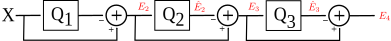
\includegraphics[width=1.0\textwidth]{figs/Proposal_fig1_RVQ_blockDiagram}
					\caption{Residual Vector Quantizer.}
					\label{fig:RVQ_blockDiagram}
			\end{figure}
			
\subsubsection{RVQ}
%-----------------
Residual Vector Quantizers were introduced by Juang et al. \cite{1982_CNF_SpeechRVQ_JuangGray}.  The RVQ structure is shown in Figure \ref{fig:RVQ_blockDiagram}.  The idea is to initially perform a crude quantization of the input vector using a small codebook.  Then a second stage quantizer operates on the error of the first quantizer.  A third quantizer may be used to quantize the second error vector, and so on.  In other words, RVQs are realized as a sequence of small ESVQs.  Each stage operates on the error vector or \emph{residual} of the preceding ESVQ \cite{1991_CNF_DesignPerformanceRVQ_Frost}.  This direct sum structure coupled with a sequential search procedure enables the RVQ to have linear rather than exponential complexity, both in computations and in memory.  

An RVQ is different from a traditional VQ in the sense that it partitions the input space $R^k$ into $M$ cells.  The residual space, also in $R^k$, is then partitioned again into $M$ cells.  This process is repeated $P$ times.  The advantage of this approach is that in obtaining $M^P$ partitions, we need to run our partitioning algorithm $P$ times and generate $M$ partitions at each stage.  In traditional VQ, the partitioning algorithm would run once but have to create $M^P$ partitions.  For the binary case (two code-vectors per stage, $M=2$) and a total of 8 stages ($P$=8), RVQ only requires 16 searches.  In $ESVQ$, this would require 256.  The exponential complexity is reduced to linear complexity.  Moreover, even the distortion of an $ESVQ$ can be attained.  In general, all structurally constrained quantizers cannot provide performance as good as ESVQ.  However, since they are able to more efficiently implement codes, larger and larger vector sizes can be used, and if carefully designed, can achieve better performance that ESVQ \cite{1996_JNL_AdvancesRVQ_Barnes}.

Another question here concerns the optimality of RVQ.  An RVQ is said to be \emph{jointly optimal} if a local or global minimum value of the average distortion $\mathcal{D}(E,D) = E[m(X_1, D(E(X_1)))]$ is achieved.  Here, $E$ is the encoder, $D$ is the decoder, $m(.,.)$ is a distortion metric, and $E[.]$ is the expectation operator.  The necessary condition for joint decoder optimality is that the code-vectors $y_p(i)$  of the $p$-th stage must satisfy the following condition:

\begin{equation}
\mathcal{D}=\frac{\partial D}{\partial y_p(i)}=0
\end{equation}

This condition is satisfied when the stage code-vectors are centroids of residuals formed from the encoding decisions of both \emph{causal} and \emph{anticausal} stages \cite{1995_JNL_OptimalityRVQ_Kossentini}.  On the other hand, if only causal stages are considered, then satisfying the condition above will help achieve \emph{sequential} optimality.  For the encoder case, it is not possible to design optimal stages.  Instead an overall global unconstrained encoder is designed, and then individual encoder stages are designed using nearest neighbor rules that try to match the performance of the global encoder.

A final note is that due to the multiple stages of RVQ, it is possible to design with few code-vectors per stage.  This can be useful if the training data is limited, since this would necessitate the use of small stage-codebook sizes \cite{1996_JNL_AdvancesRVQ_Barnes}.

Having discussed optimality conditions and general design guidelines of RVQ, we now turn our attention to the usage of RVQ as a classifier.  It is in this role that we seek to use it for our multi-target tracking problem.

\subsubsection{RVQ as a Classifier}
%------------------------------
The usage of RVQ as a classifier was reported in Barnes \cite{2007_JNL_IDDM_Barnes} in the context of image driven data mining.  In this work, a $\sigma$-tree is used as a data structure for RVQ stage code-vectors.  To better understand the $\sigma$-tree classifier, we relate it with other well-known areas of information theory,
pattern recognition and machine learning:  

\begin{itemize}
\item The $\sigma$-tree classifier is a type of variable rate vector quantizer \cite{2003_JNL_HighRateVQDetection_Hero}.  

\item Truncel et al. explore the relationship between rate-distortion theory and content-based retrieval in high dimensional databases \cite{2004_JNL_RateDistortionVsDatabases_Truncel}.  

\item The $\sigma$-tree design problem parallels the joint codebook design problem addressed in the source coding literature for multiple stage vector quantization \cite{1996_JNL_AdvancesRVQ_Barnes}.  

\item The $\sigma$-tree classifier can be compared to dimensionality reduction methods such as Principal Components Analysis (PCA).  PCA seeks to reorient the basis vectors in $R^k$ and achieves compression by ignoring projected data components with least variances.  A $\sigma$-tree classifier achieves compression by encoding a source symbol with a lower dimensional tuple.

\item The $\sigma$-tree classifier partitions the decision space $R^k$ like other well known classifiers such as neural networks and support vector machines \cite{2007_JNL_IDDM_Barnes}.  Further, note that neural networks partition the decision space with hyperplanes or hypersurfaces, depending on whether or not hidden layers are used.  Support vector machines also partition the decision space, but with maximum margin hyperplanes in a higher dimensional space.  The $\sigma$-tree classifier tessellates the decision space $R^k$ with $k$ Voronoi cells.  In $R^2$, Voronoi cells are the geometric dual of delaunay triangulation.  

\item As already discussed, the Linde Buzo Gray (LBG) algorithm is widely used to design the encoder and decoder of a VQ, including RVQ and the $\sigma$-tree classifier.  This algorithm is similar to the well-known $k$-means algorithm \cite{1967_CNF_Kmeans_Macqueen}.

\item The stage indices returned by the $\sigma$-tree classifier can be used to probabilistically determine class membership, similar to the probabilistic output of Relevance Vector Machines \cite{2001_JNL_RVM_Tipping} or Probabilistic Neural Networks \cite{1990_JNL_PNN_Specht}.  The multiple stages of the $\sigma$-tree classifier suggest a coarse to fine classification route, i.e., successive approximations.
\end{itemize}

Having discussed tracking and RVQ in detail, we now turn to our prior research in these areas.



			\begin{figure}		
					\centering		
					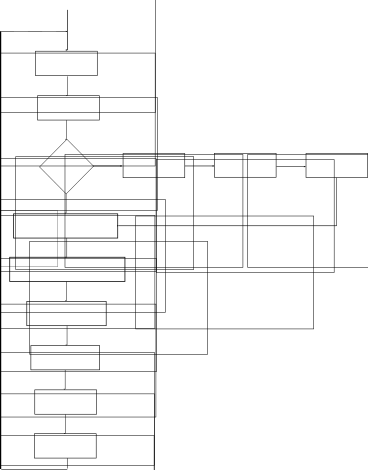
\includegraphics[width=0.5\textwidth]{figs/Proposal_fig2_RVQ_MTT_BlockDiagram}
					\caption{Multi-target tracking using RVQ.}
					\label{fig:MTT_BlockDiagram}
			\end{figure}

%##############################################################################################################
\newpage
\section{Preliminary Research}
\label{Sec:Preliminary}
%##############################################################################################################
Our work reports the first usage of RVQ for any form of video analysis.  The preliminary research that forms the basis of this work is based on the following 8 components:

\begin{enumerate}
\item RVQ used in video tracking
\item RVQ used for human action recognition
\item Region based tracking
\item Contour based tracking
\item Background modeling
\item Video stabilization (patent applied)
\item Feature extraction (related to patent work)
\item Analytical approximation to a quantizer function 
\end{enumerate}
  
			\begin{figure}		
					\centering		
					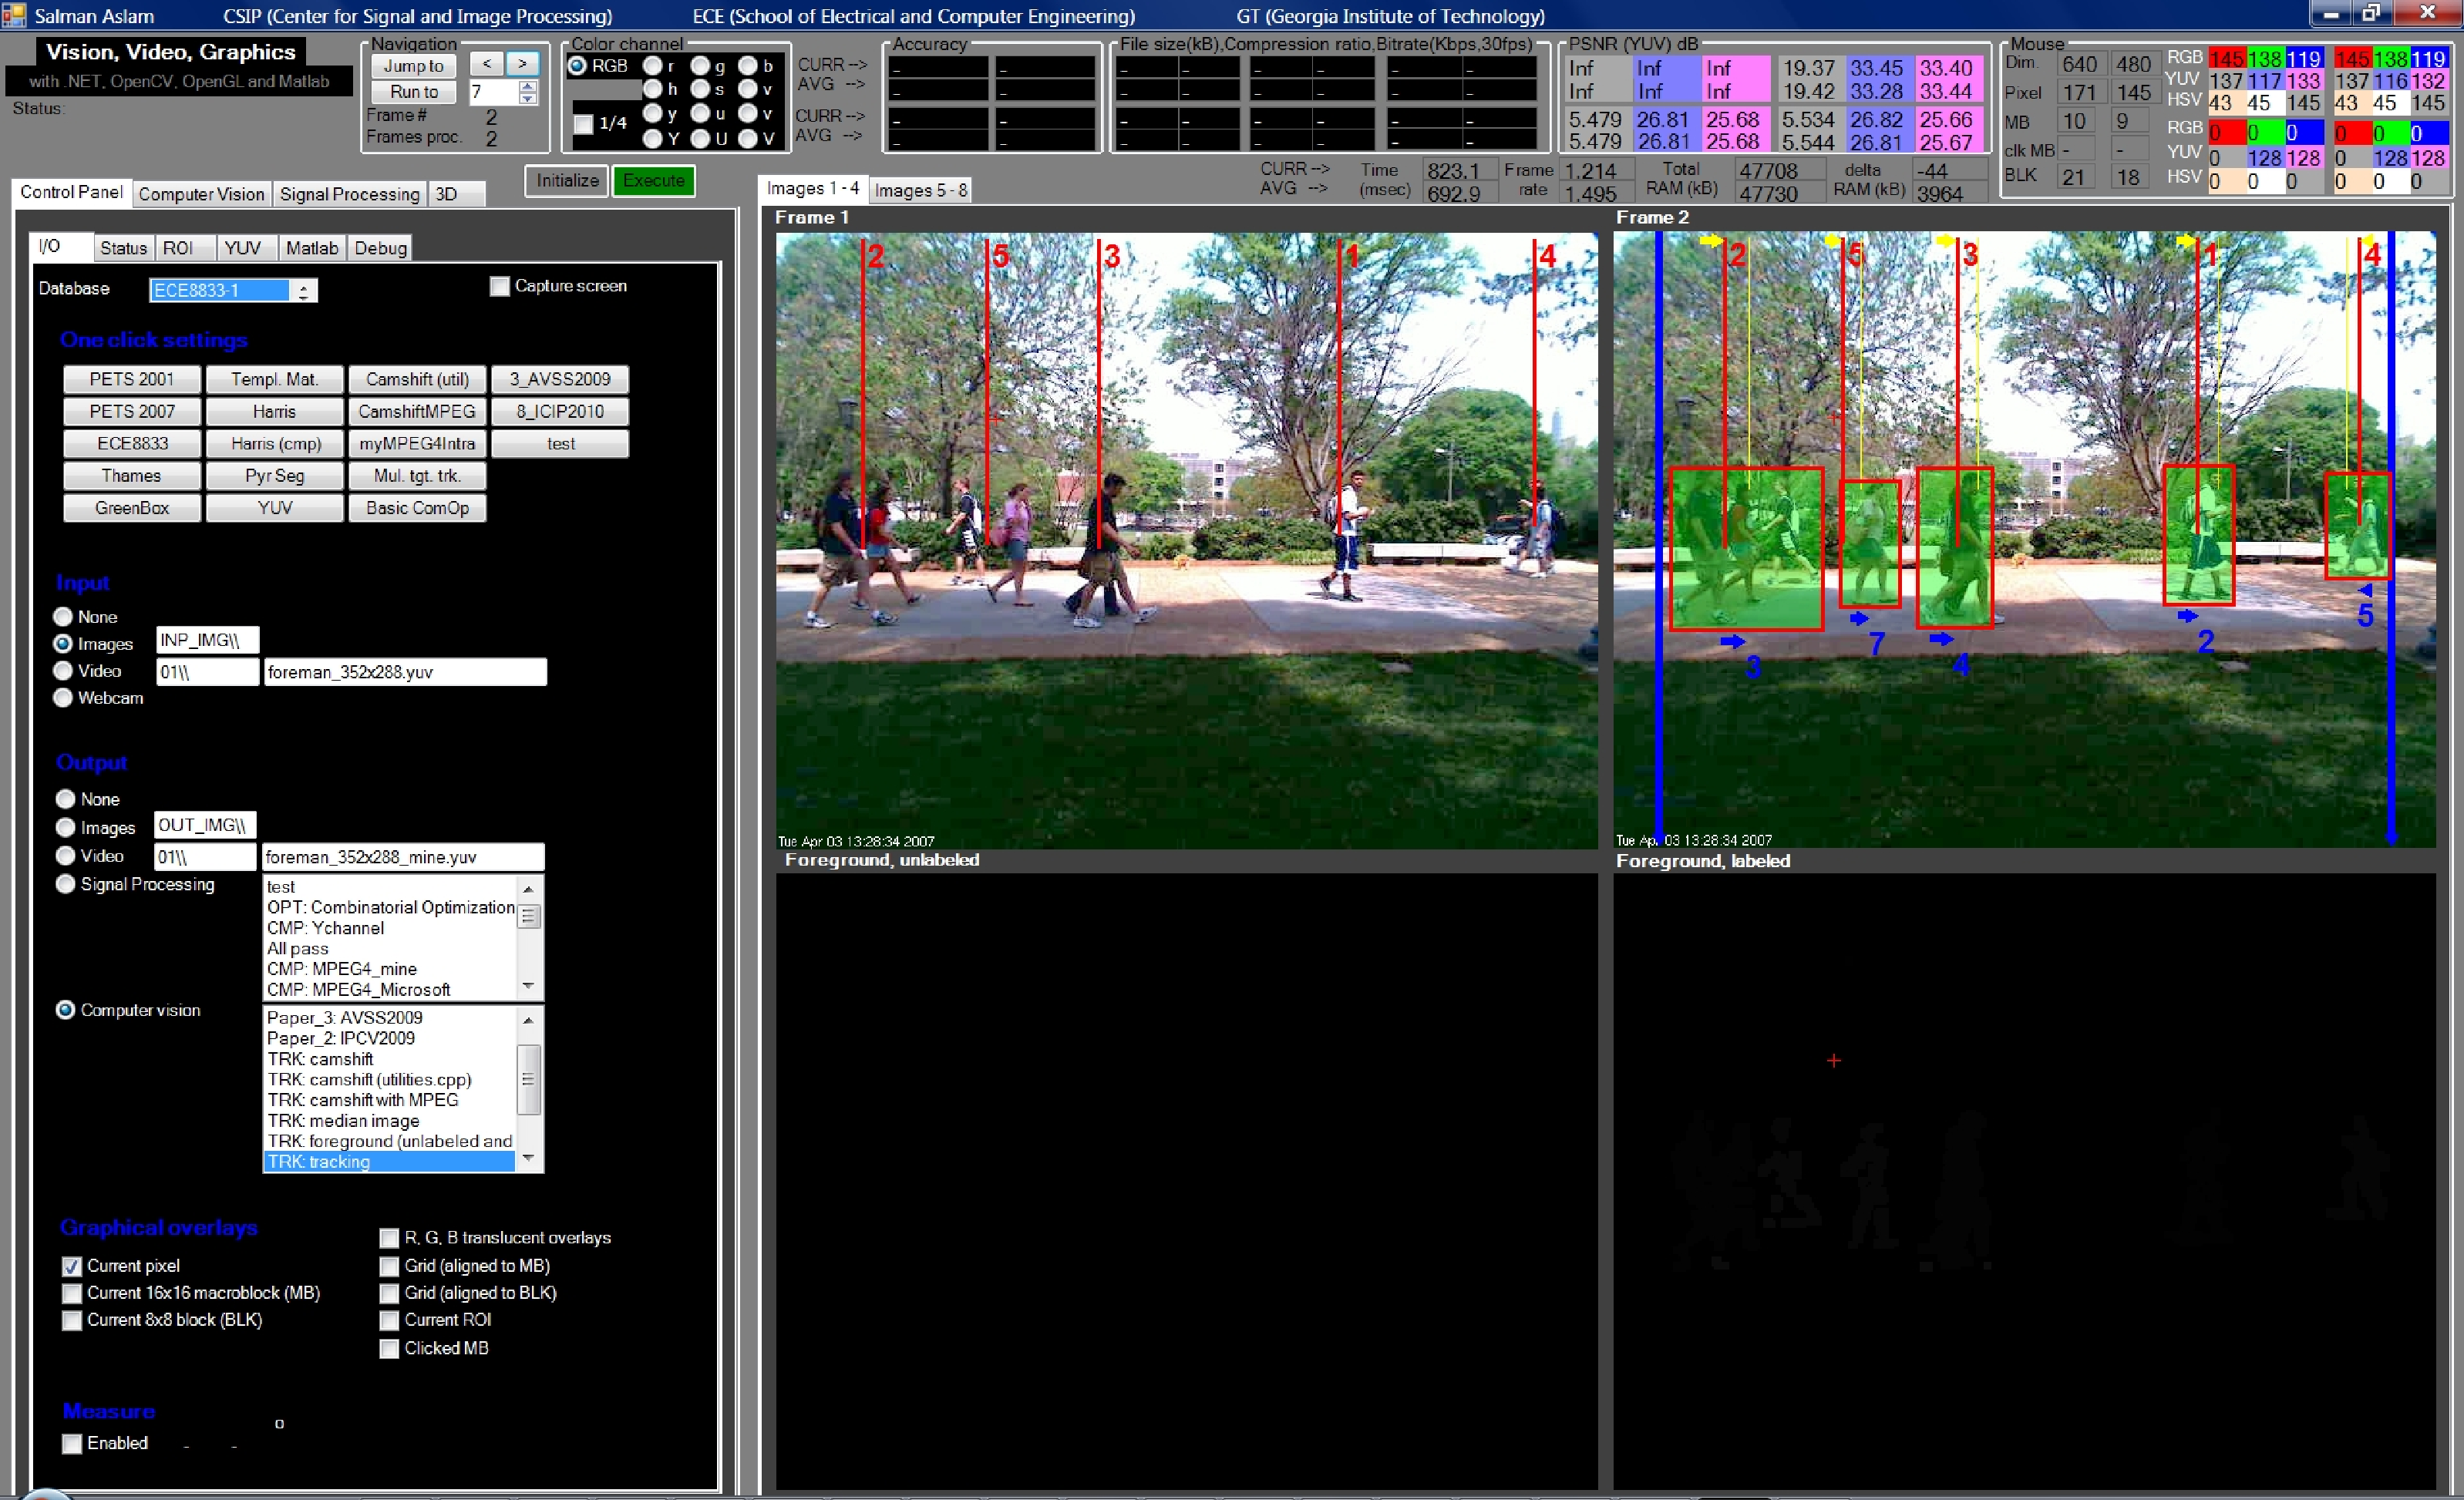
\includegraphics[width=1.0\textwidth]{figs/Proposal_fig3_RVQ_MTT_snapshot_VVG}
					\caption{Snapshot of the tracking scenario.}
					\label{fig:snapshot_VVG}
			\end{figure}	
			

We now present details of this preliminary work. 
			
\subsection{RVQ: Target Tracking}
%================================
In this work, we track multiple targets using RVQ as a classifier-detector.  This approach of combining tracking with a classifier-detector has been used by other researchers.  For instance, Lipton et al. \cite{1998_CNF_Tracking_Lipton} use unsupervised learning to train a maximum likelihood classifier.  This classifier is subsequently used to classify targets as car or human.  Avidan \cite{2004_JNL_SVMtracking_Avidan} uses a trained SVM classifier to detect cars.  This detection step augments an optical flow tracker. 
 
			\begin{figure}%[htp]
						\centering	
						\subfigure[Decoder codebooks.]
						{
							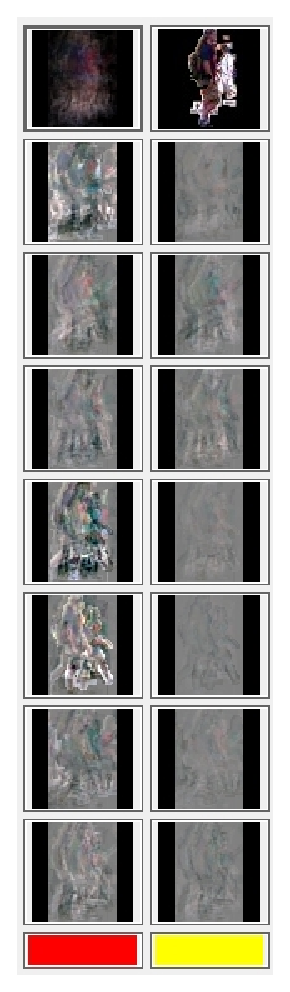
\includegraphics[width=0.15\textwidth]{figs/Proposal_fig4a_RVQ_MTT_codebooks}
							\label{fig:MTT_codebooks}	
						}
						\subfigure[Target reconstruction using the decoder codebooks.]
						{
							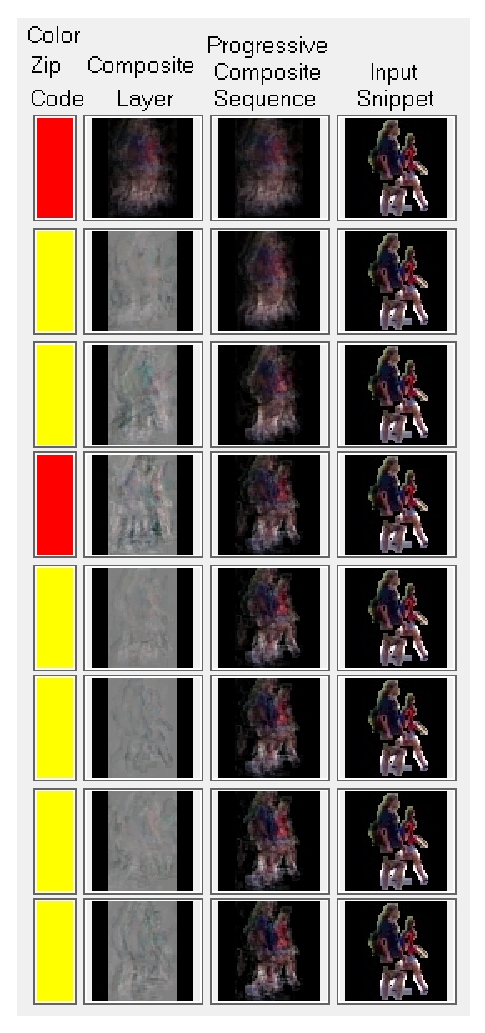
\includegraphics[width=0.23\textwidth]{figs/Proposal_fig4b_RVQ_MTT_reconstruction}
							\label{fig:MTT_reconstruction}	
						}
						\caption{Multi-target tracking, codebooks and reconstruction.} 
						\label{fig:Codebooks_and_reconstruction}				
			\end{figure}
						
A block diagram of our approach is shown in Figure~\ref{fig:MTT_BlockDiagram}.  A sample tracking scenario is shown in Figure~\ref{fig:snapshot_VVG}.  We track several targets in a dense environment.  Background maintenance is done using a multi-gaussian background subtraction algorithm.  Track initialization is done using template matching.  Multiple instances of each target are used to train one set of encoder and decoder codebooks per target.  Subsequent foreground objects are tested against every codebook.  The codebook that most explains the target is chosen for association.
			
A few details about the RVQ parameters are now presented.  Figure~\ref{fig:MTT_codebooks} shows the direct sum code-vectors of the decoder codebook.  We use 2 code-vectors per stage ($N=2$), and a total of 8 stages ($P=8$).  Although this number is somewhat arbitrary, empirical analysis shows that this is a reasonable setting.  A total of $N^P$, or 256 unique images can be represented with this codebook, but the computational cost of computation and storage is $O(NP)$ rather than $O(N^P)$.  Once the codebooks have been created for time $t=1$ to $t=T$, subsequent targets at times $t=T+1, T+2, \ldots$ are encoded using the codebooks.  The codebook that results in the least reconstruction error is chosen and the target corresponding to that codebook is matched.  Figure~\ref{fig:MTT_reconstruction} shows reconstruction of a target using the codebooks.  

The software used for this research is shown in Figure~\ref{fig:snapshot_VVG}.  A .NET framework was integrated with Matlab, Intel OpenCV and OpenGL for mathematical, image processing and visualization purposes.  

			\begin{figure}		
			\centering		
					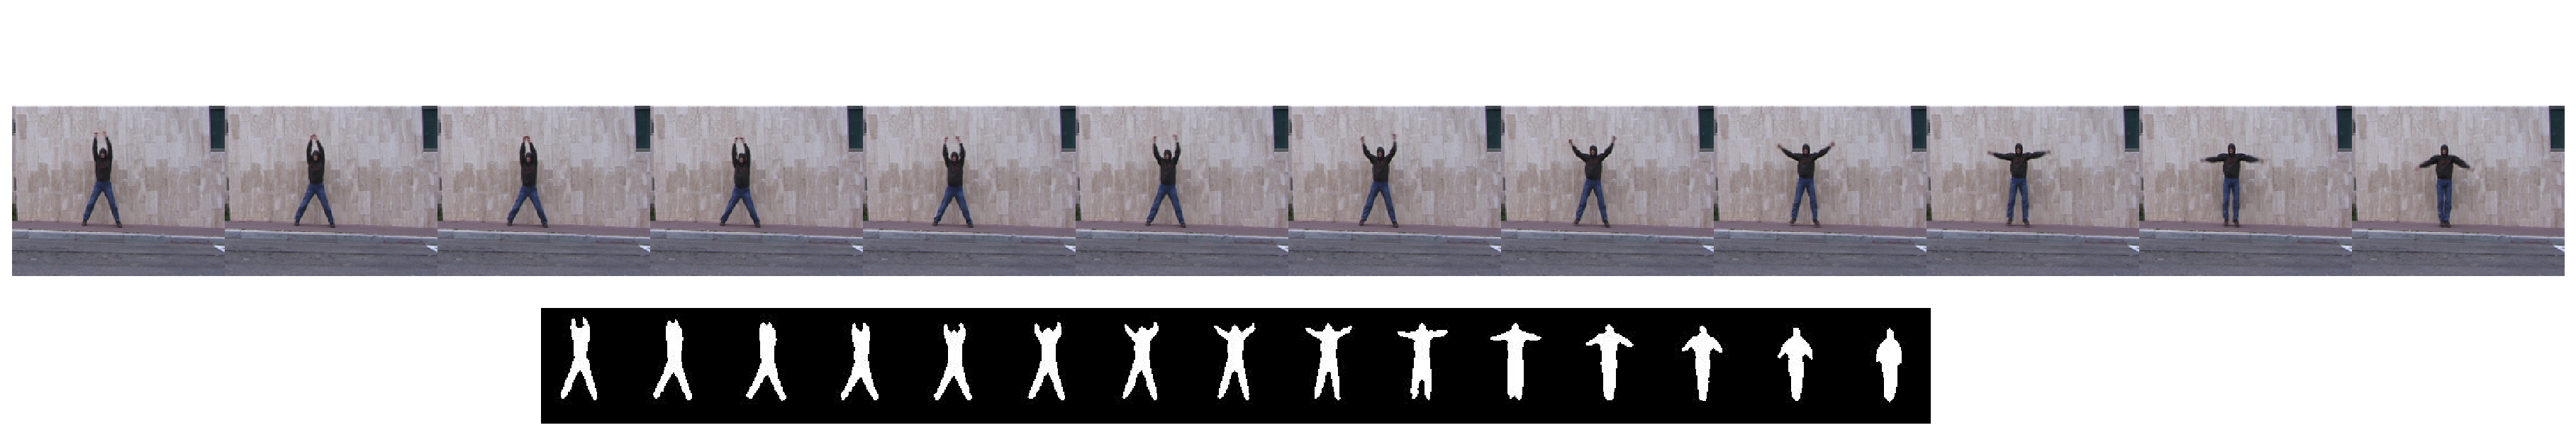
\includegraphics[width=1.0\textwidth]{figs/Proposal_fig5_RVQ_HMM_Weizmann_dataset}
					\centering
					\caption{Sample images from the Weizmann dataset.}
					\label{fig:Weizmann_sequence}
			\end{figure}
			

\subsection{RVQ: Human Action Recognition}
%=========================================
The second phase of our experimentation with RVQ is based on human action recognition \cite{2010_CNF_HMMRVQ_Aslam}.  The area of human action recognition has recently received a lot of attention.  A number of surveys are available on this topic \cite{1995_JNL_SURVEYmotion_Cedras,1999_JNL_SURVEYmotion_Aggarwal,1999_JNL_SURVEYmotion_Gavrila,1999_REP_SURVEYmotion_Moeslund,2001_JNL_SURVEYmotion_Moeslund,2003_JNL_SURVEYiu_Buxton,2003_JNL_SURVEYmotion_LWang,2003_JNL_SURVEYbeh_Shah,2003_JNL_SURVEYmotion_Wang,2004_CNF_SURVEYaction_Aggarwal,2004_JNL_SURVEYiu_Hu,2004_CNF_SURVEYgait_Nixon,2004_CNF_Survey3DshapeRetrieval,2006_JNL_HumanMotion_Moeslund,2007_JNL_HumanMotion_Poppe,2008_CNF_SurveyHumanActivityRecognition_Ahad,2010_JNL_SURVEYmotion_Ji}.  Bobick et al. \cite{2001_JNL_MotionTemplates_Bobick} introduced the notion of 2D templates of human action.  This was extended to 3D by Gorelick et al. \cite{2007_JNL_SpaceTimeShapes_Gorelick}.  Recently an approach based on kinematic features of 3D motion was used to recognize human action \cite{2010_JNL_ActionReconKinematic_Ali}.  Our approach to tackling this problem is similar to \cite{2007_JNL_SpaceTimeShapes_Gorelick} in the sense that extracted features are used for classification using a simple Euclidean distance measure.  We use a four step approach:  

			\begin{figure}%[htp]
						\centering	
						\subfigure[Decoder codebooks.  With 2 code-vectors per stage, and 8 stages, a total of 256 reconstructed images are possible.  With 3 code-vectors per stage, a total of 6561 reconstructed images are possible.]
						{
							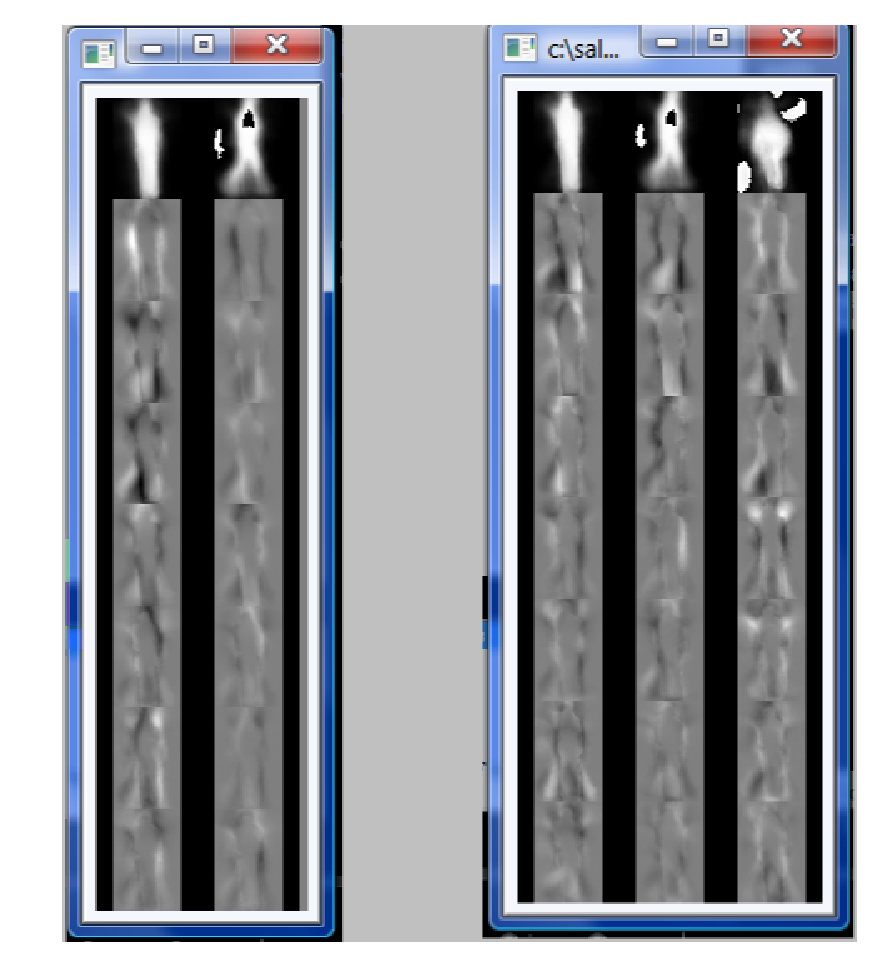
\includegraphics[width=.50\textwidth]{figs/Proposal_fig6a_RVQ_HMM_Weizmann_codebooks}
							\label{fig:Weizmann_codebooks}	
						}
						\hspace{1in}
						\subfigure[Image reconstruction using the decoder codebooks.]
						{
							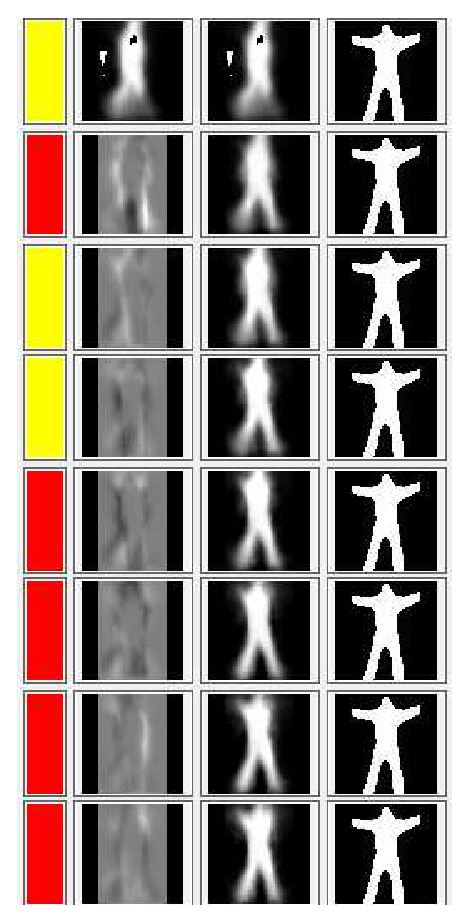
\includegraphics[width=0.25\textwidth]{figs/Proposal_fig6b_RVQ_HMM_Weizmann_reconstruction}
							\label{fig:Weizmann_reconstruction}	
						}
						\caption{Human action recognition, codebooks and reconstruction.} 
						\label{fig:Weizmann_codebooks_and_reconstruction}				
			\end{figure}
			
\begin{enumerate}			
\item In the first step, we separate the dataset shown in Figure \ref{fig:Weizmann_sequence} into training and test images using the leave one out method \cite{2000_JNL_SURVEYprml_Jain}.  RVQ codebooks, shown in Figure~\ref{fig:Weizmann_codebooks}, are generated using this training set.  This one time offline step takes approximately 6 minutes for 2400 images on a Core2 Duo 2.5 GHz laptop.  

\item In the second step, a descriptor $x_i$ is generated for each of the $i$ training images using the decoder codebooks.  The first stage is weighted the most, followed by geometrically decreasing weights for the subsequent stages.  For $M$ code-vectors per stage and a total of $P$ stages, the descriptor, $x_i$ is a geometric sum given by,

\begin{equation}
x_i=\sum_{p=0}^{P-1}a_pM^{(P-1-p)}
\end{equation}

Notice that for 2 code-vectors per stage, the descriptor ranges from 0 to 255, and a single byte is required to represent an entire image.  These training image descriptors can be used for classification in a manner similar to the training image projections in PCA analysis.  The RVQ based descriptors or PCA based projections can be used to create class conditional densities.  These densities can then be used for classification using maximum likelihood, or maximum aposteriori methods.  The processing time to create training image descriptors is about 3 minutes.  However, it is also an offline step.  The processing time includes GUI related instructions as well as SQL Server database access times.

			\begin{figure}
						\centering	
						\subfigure[Our method \cite{2010_CNF_HMMRVQ_Aslam}]
						{
							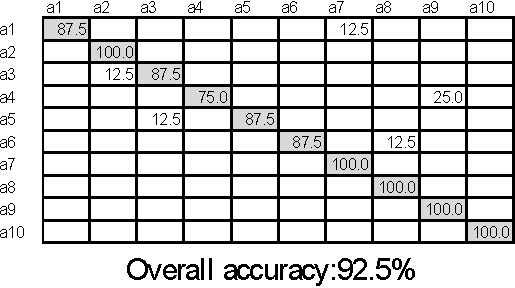
\includegraphics[width=.50\textwidth]{figs/Proposal_fig7a_RVQ_HMM_Weizmann_TabularResults_us}
							\label{fig:Weizmann_TabularResults_us}	
						}
						\subfigure[Gorelick et al. \cite{2007_JNL_SpaceTimeShapes_Gorelick}]
						{
							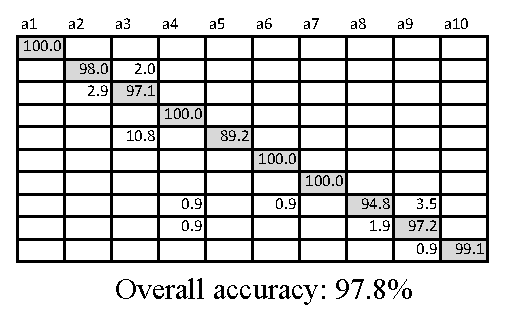
\includegraphics[width=0.45\textwidth]{figs/Proposal_fig7b_RVQ_HMM_Weizmann_TabularResults_gorelick}
							\label{fig:Weizmann_TabularResults_gorelick}	
						}
						\subfigure[Manor et al. \cite{2001_CNF_EventBasedAnalysisVideo_Manor}]
						{
							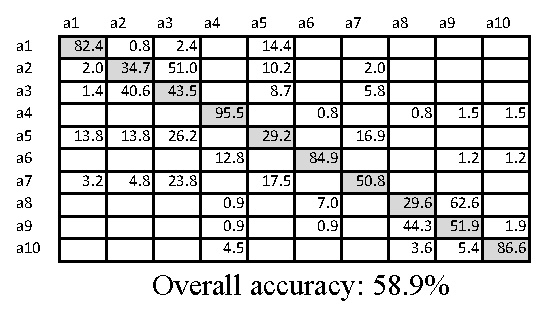
\includegraphics[width=0.50\textwidth]{figs/Proposal_fig7c_RVQ_HMM_Weizmann_TabularResults_manor}
							\label{fig:Weizmann_TabularResults_irani}	
						}
						\subfigure[Ali et al. \cite{2010_JNL_ActionReconKinematic_Ali}]
						{
							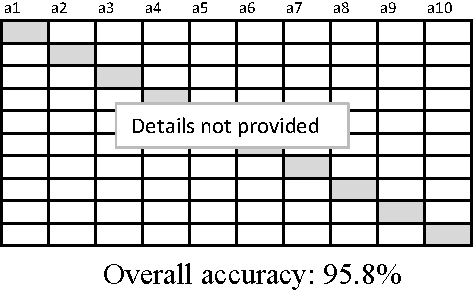
\includegraphics[width=0.45\textwidth]{figs/Proposal_fig7d_RVQ_HMM_Weizmann_TabularResults_shah}
							\label{fig:Weizmann_TabularResults_shah}	
						}												
						\caption{Human action recognition, action confusion matrix.} 
						\label{fig:Weizmann_TabularResults}				
			\end{figure}
						
\item In the third step, an HMM is trained on the descriptor evolution for every action sequence in the training set.  The 10 actions available are walk (a1), run (a2), skip (a3), jumping jacks (a4), jumping (a5), in-place jumping (a6), sideways motion (a7), waving with one hand (a8), waving with two hands (a9) and bending (a10).  There are a total of 8 users.  This step takes around 700 msec in Matlab.  All previous steps were executed in the C language.

\item In the fourth step, descriptor sequences are generated for the test images and tested against each HMM action model.  The model that best represents an action is picked.  This step is then repeated for all users in the database using the leave one out procedure.  This step takes 1.1 msec per frame in Matlab.   
\end{enumerate}

			%contours
			\begin{figure}[t]
						\centering
			
						\subfigure[]
							{
								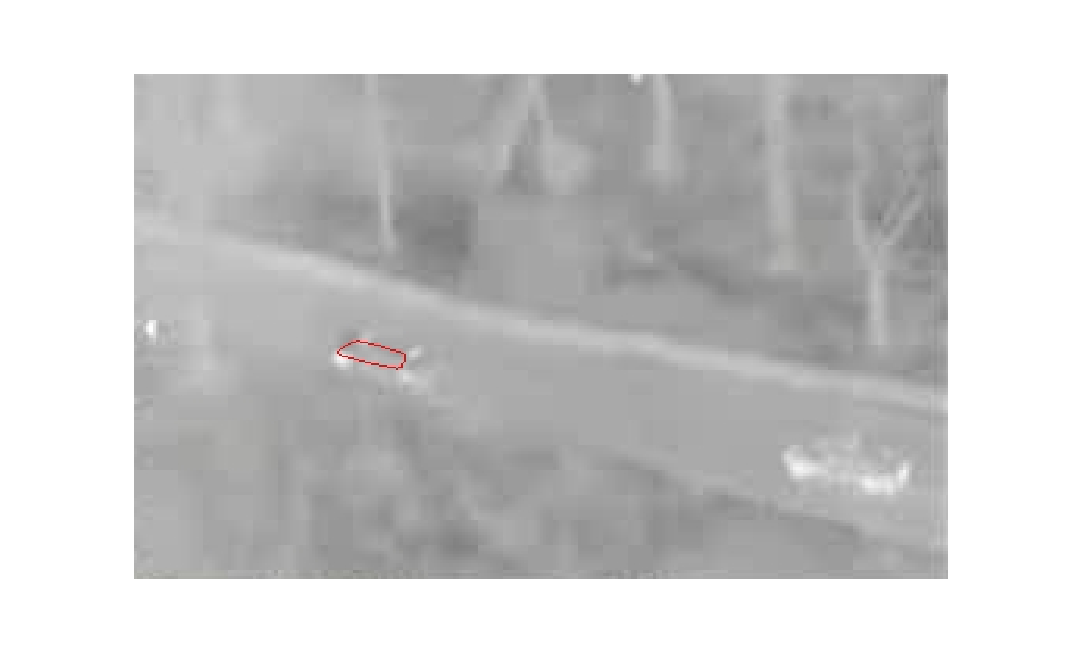
\includegraphics[width=.46\textwidth]{figs/Proposal_fig8a_TRK_CONTOUR_PoliceIR_FN_00030}
								\label{subfig:1250}
							}
						\subfigure[]
							{
								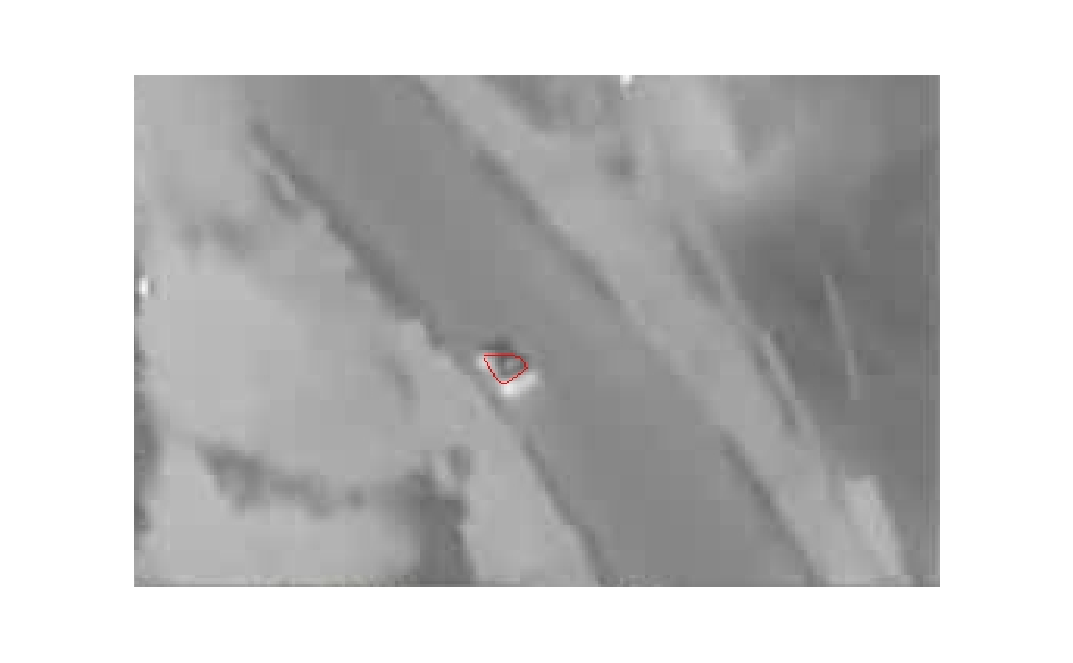
\includegraphics[width=.45\textwidth]{figs/Proposal_fig8b_TRK_CONTOUR_PoliceIR_FN_01277}
								\label{subfig:01277_contour}
							}								
						\caption{Contour tracking.} 	
						\label{fig:Contours}	
			\end{figure}

We compare our results in Figure \ref{fig:Weizmann_TabularResults} with other researchers who have used the same database for exactly the same human action recognition purposes.  It may be noted that our results are based on using only 40\% of the training images.  The reason for not using the entire dataset is that each action has a different number of images in the database.  We have used an equal number of 25 images per action corresponding to half a second of video.  It is expected that if 1 second clips are used for all actions, our results will improve.  Unfortunately, at this point, this dataset does not have 1 sec clips for all actions.  


					\begin{figure}
					\centering
					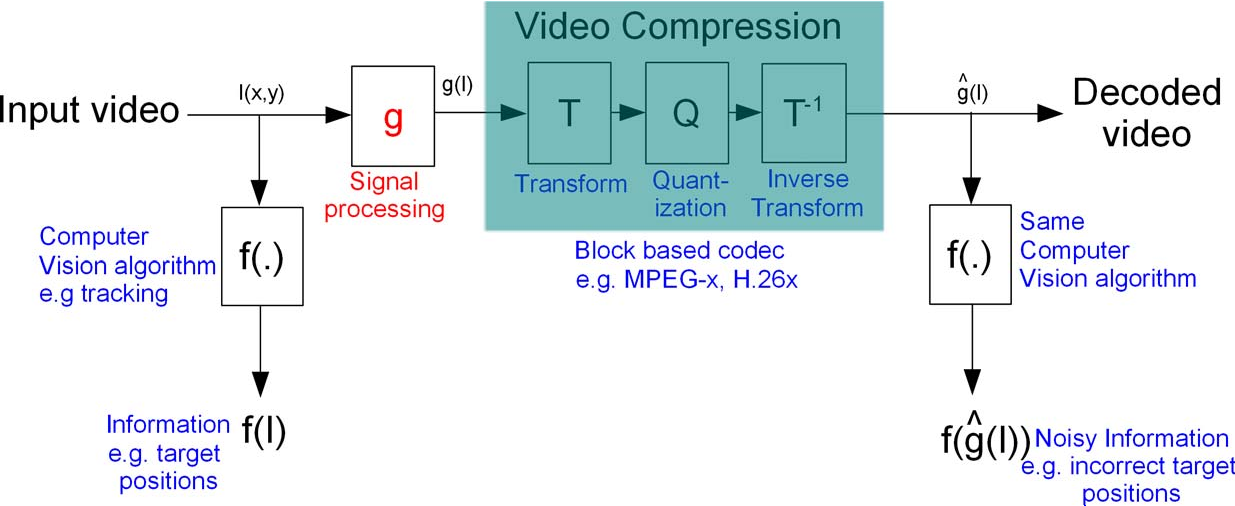
\includegraphics[width=0.75\textwidth]{figs/Proposal_fig9_TRK_lowBitrate_blockDiagram}
					\caption{Kernel tracking on low bit rate video, block diagram}
					\label{fig:SolutionThroughSigProc2}
					\end{figure}



						\begin{figure}
						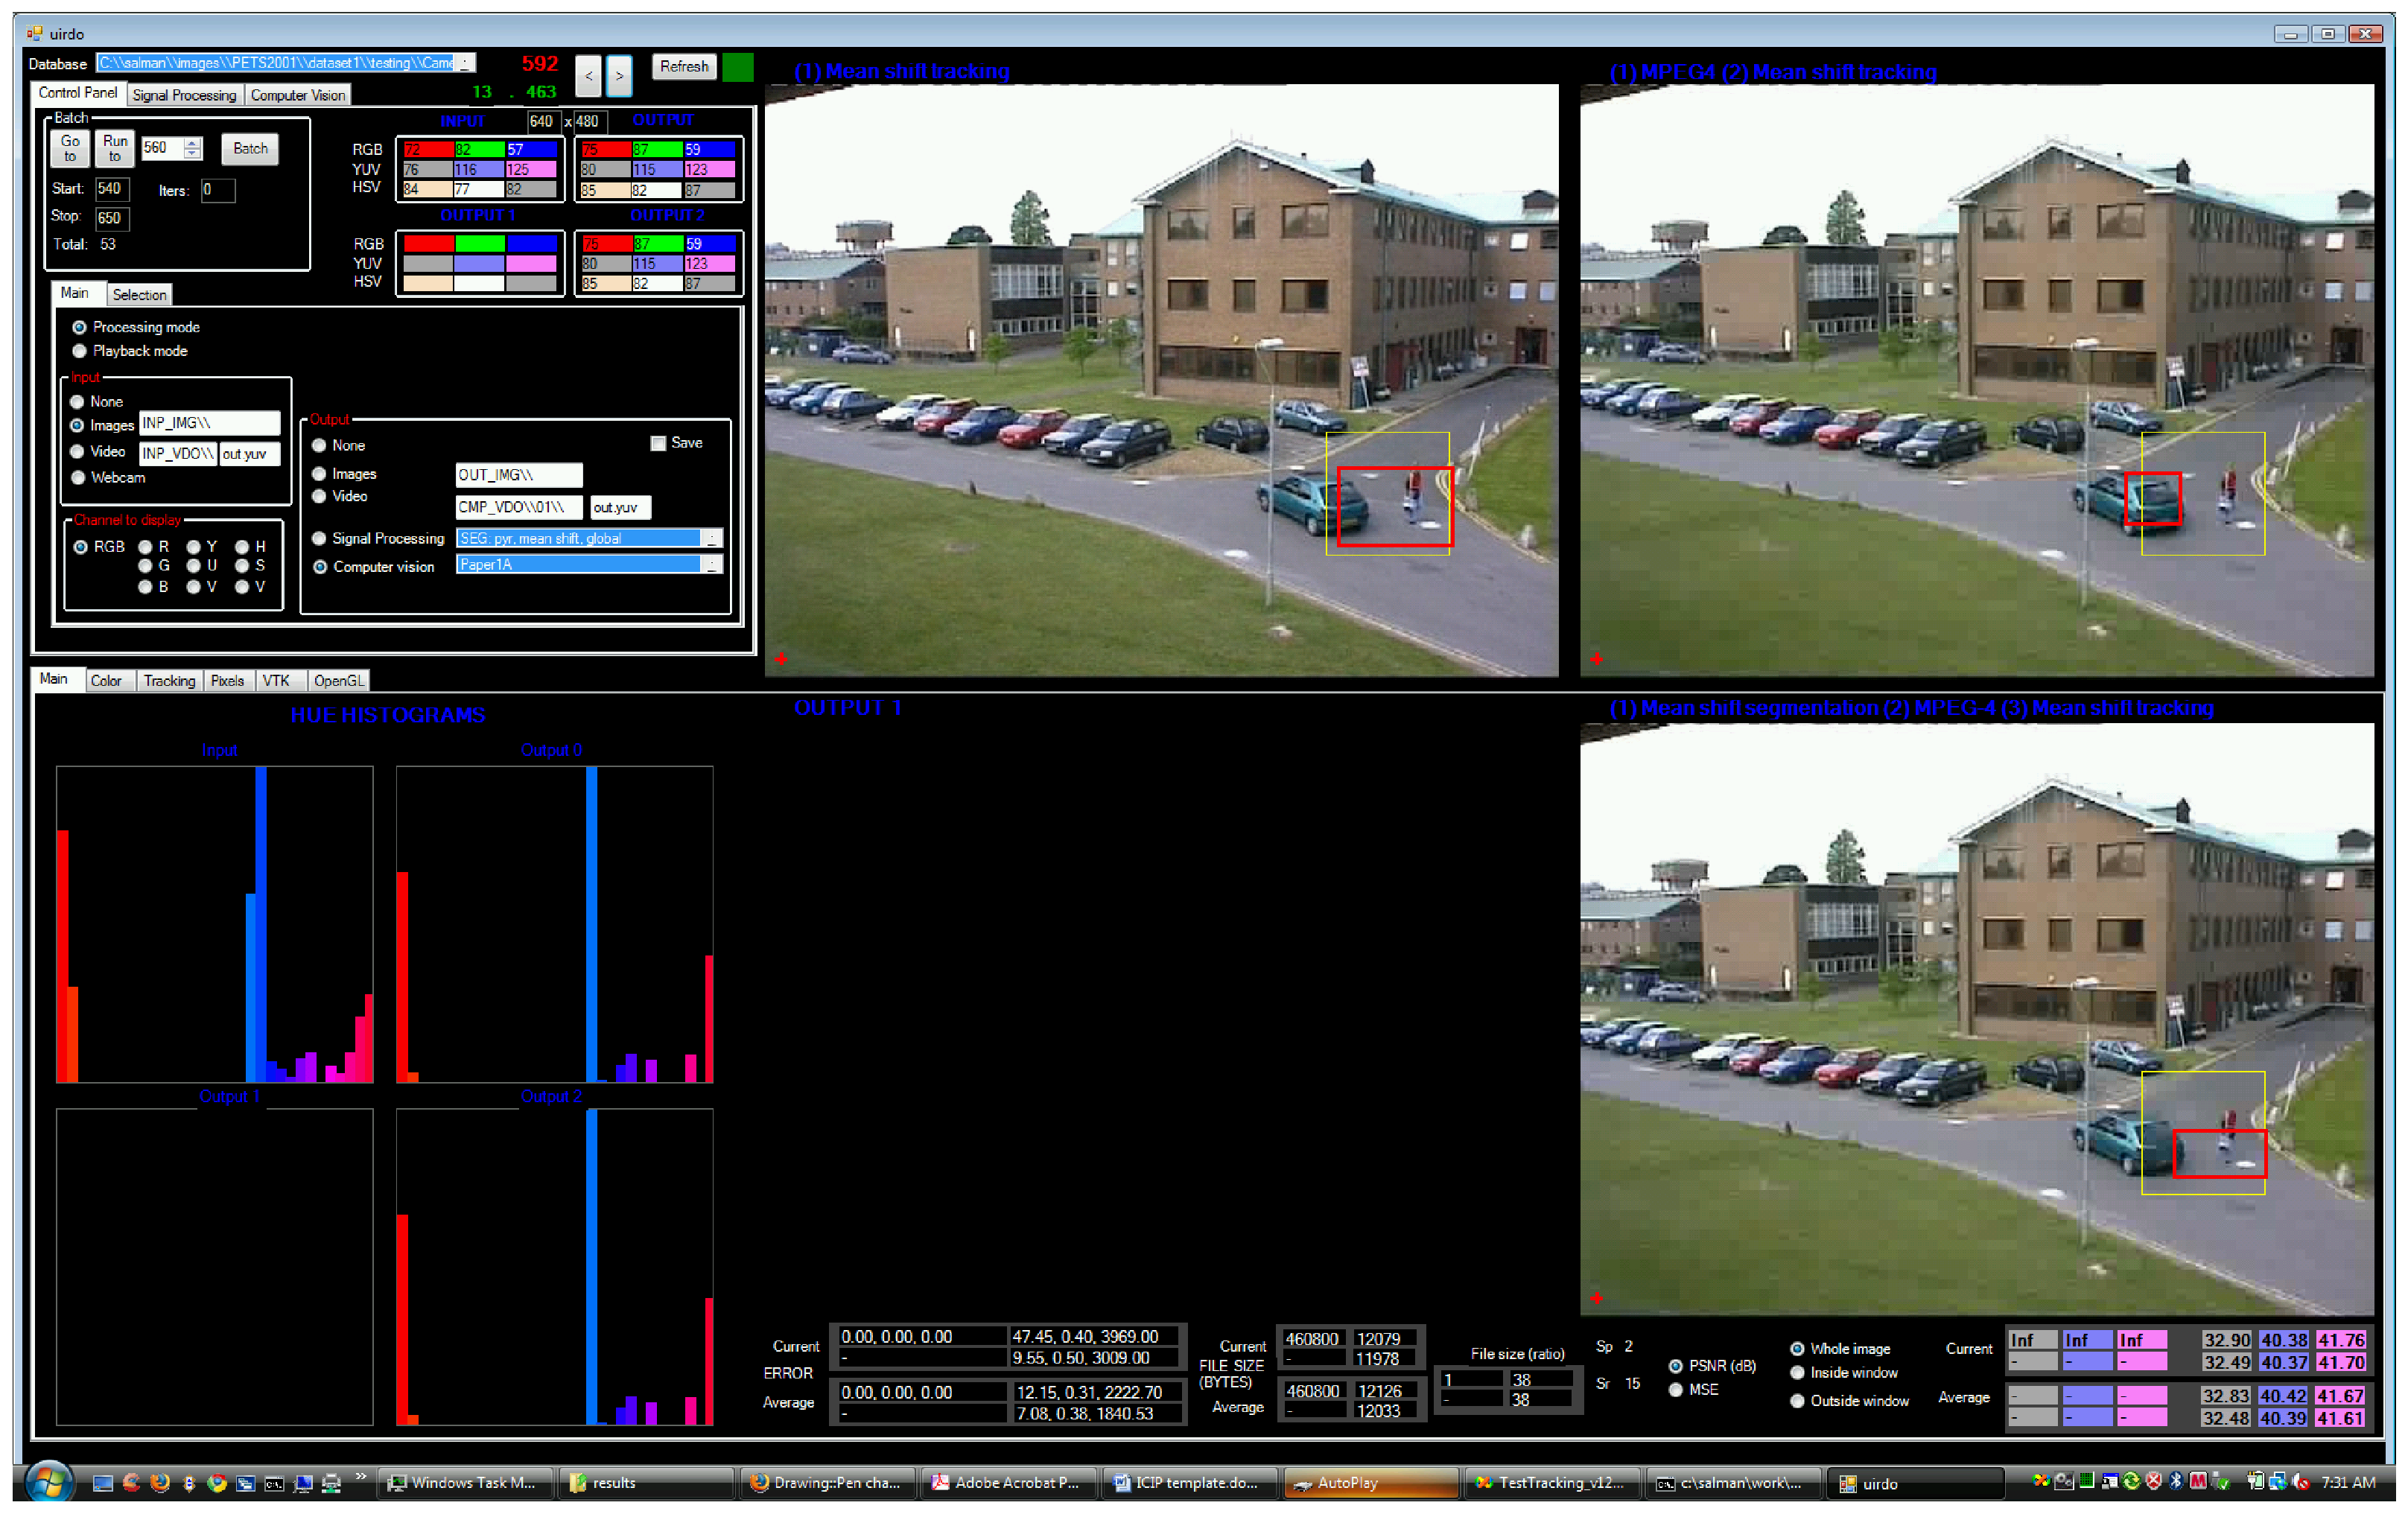
\includegraphics[width=1.0\textwidth]{figs/Proposal_fig10_TRK_lowBitrate_PETS2001_FN_592}
						\label{fig:KernelTracking_picture}
						\caption{Kernel tracking on low bit rate video, compensated signal holds track.}
						\end{figure}

			
\subsection{Tracking: Contour Tracking on Low Contrast Video}
%============================
Having discussed preliminary work on RVQ and its application in multi-target tracking and human action recognition, we now turn to some preliminary work related to tracking alone.  Recall that RVQ uses appearance information.  In this work, we experiment with contour based tracking \cite{2010_CNF_VehicleContour_Aslam}.  Our work is similar to Yilmaz et al. \cite{2003_JNL_AirborneIRtracking_Yilmaz}.  Whereas they use global motion compensation and mean-shift for region tracking, we use interest-point matching followed by elliptical fourier descriptors for contour tracking.  Elliptical fourier descriptors have been explained in Section \ref{Sec:Origin}.

The idea behind this work is that certain targets demonstrate typical specular points in the IR domain.  For vehicles, these points can result at the tires due to the heat generated from friction.  Luckily, these points can be detected as strong corners.  Moreover, these points appear at the edges of the vehicle.  This allows us to draw a contour around the vehicle of interest using elliptical fourier descriptors \cite{1982_JNL_EllipticalFourier_Kuhl}.  The result is robust, real-time, contour tracking on vehicles acquired from IR acquisition systems.  Figure \ref{fig:Contours} shows an example of our approach.  

						\begin{figure}
						\centering
						\subfigure[Block diagram.]
							{
								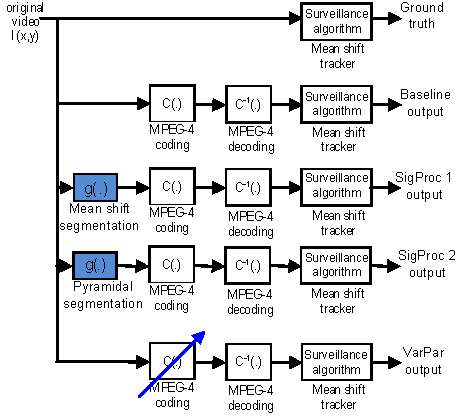
\includegraphics[width=.45\textwidth]{figs/Proposal_fig11a_TRK_lowBitrate_experimentalSetup}
								\label{fig:ExperimentalSetup}
							}	
						\subfigure[Overall Tracking performance over all possible bit rates.]
							{
								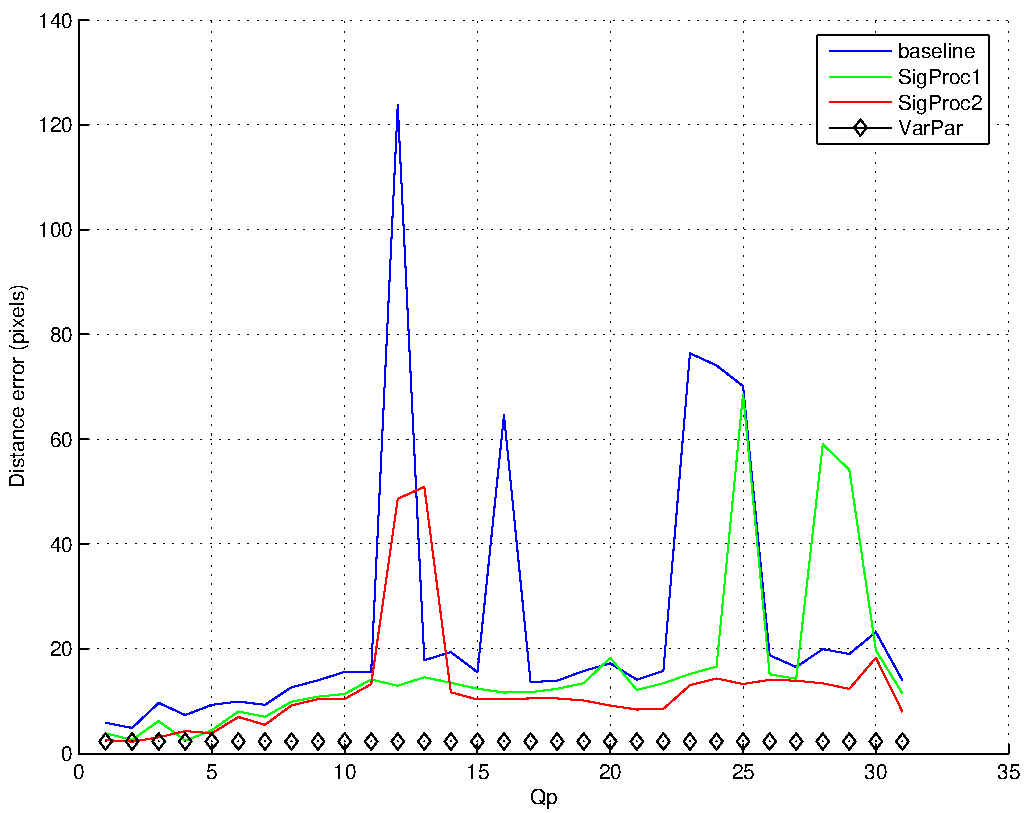
\includegraphics[width=.45\textwidth]{figs/Proposal_fig11b_TRK_lowBitrate_PETS2001_accuracyAllQp}
								\label{fig:KernelTracking_Results}
							}										
							\caption{Kernel tracking on low bit rate video, experimental setup.} 	
						\label{fig:KernelTracking_ExperimentalSetup}	
						\end{figure}


\subsection{Tracking: Region Density Tracking on Low Bit Rate Video}
%===========================================================
Having described some preliminary work on contour tracking, we now turn to region tracking.  In this work, our goal is to find a general methodology to preserve the performance of a computer vision algorithm running on compressed video \cite{2009_CNF_CVcompMS1_Aslam}.  The particular computer vision algorithm that we choose to work with is region tracking, and in particular, mean-shift tracking on color density represented in the HSV domain \cite{2002_JNL_MeanShift_Comaniciu}.  We start quite generally and cast this problem as a calculus of variations problem:

\begin{equation}
	\label{eq:CalcOfVarFormulation}
  \min_{g} J(g)=\int\int_D \left\|f(I) - f(\hat{g}(I)) \right\|_2  +  \lambda \left\|p(I) -  p(\hat{g}(I)) \right\|_2 dxdy
\end{equation}

This is to say that over the space of all signal processing transformations $g(I)$ that can be applied to the input image $I(x,y)$, we would like to find the transformation that minimizes the distance between the output of a computer vision algorithm $f(I)$ running on the original and compressed images.  At the same time, we would also like maximize some similarity measure $p(I)$ of the image.  In this case, the computer vision algorithm $f(I)$ is mean-shift tracking.  It is clear that Equation~\ref{eq:CalcOfVarFormulation} is not differentiable due to the discontinuities on the $kxk$ DCT block boundaries, assuming of course that we are using a block-based codec such as MPEG-x or H.26x (we assume intra-coding without loss of generality).  However, even if numerical schemes are resorted to, the Euler Lagrange approach to solving the variational problem is a necessary but not sufficient condition for global optimality.  This problem is depicted graphically in Figure \ref{fig:SolutionThroughSigProc2}.  Our solutions, depicted as $SigProc1$ and $SigProc2$ in Figure \ref{fig:KernelTracking_ExperimentalSetup} include iteratively adjusting the color density of the input video $I$ using a greedy algorithm so that a local minimum in tracking error is achieved.  Another approach $VarPar$ achieves low tracking error by iterating over possible $Q_p$ (quantization parameter) values.  Comparative performance of these algorithms in Figure \ref{fig:KernelTracking_Results} shows that over all values of $Q_p$, i.e. all possible bit rates, all our methods outperform the baseline tracker.

\subsection{Pre-processing: Background Modeling}
%===============================================
			\begin{figure}		
					\centering		
					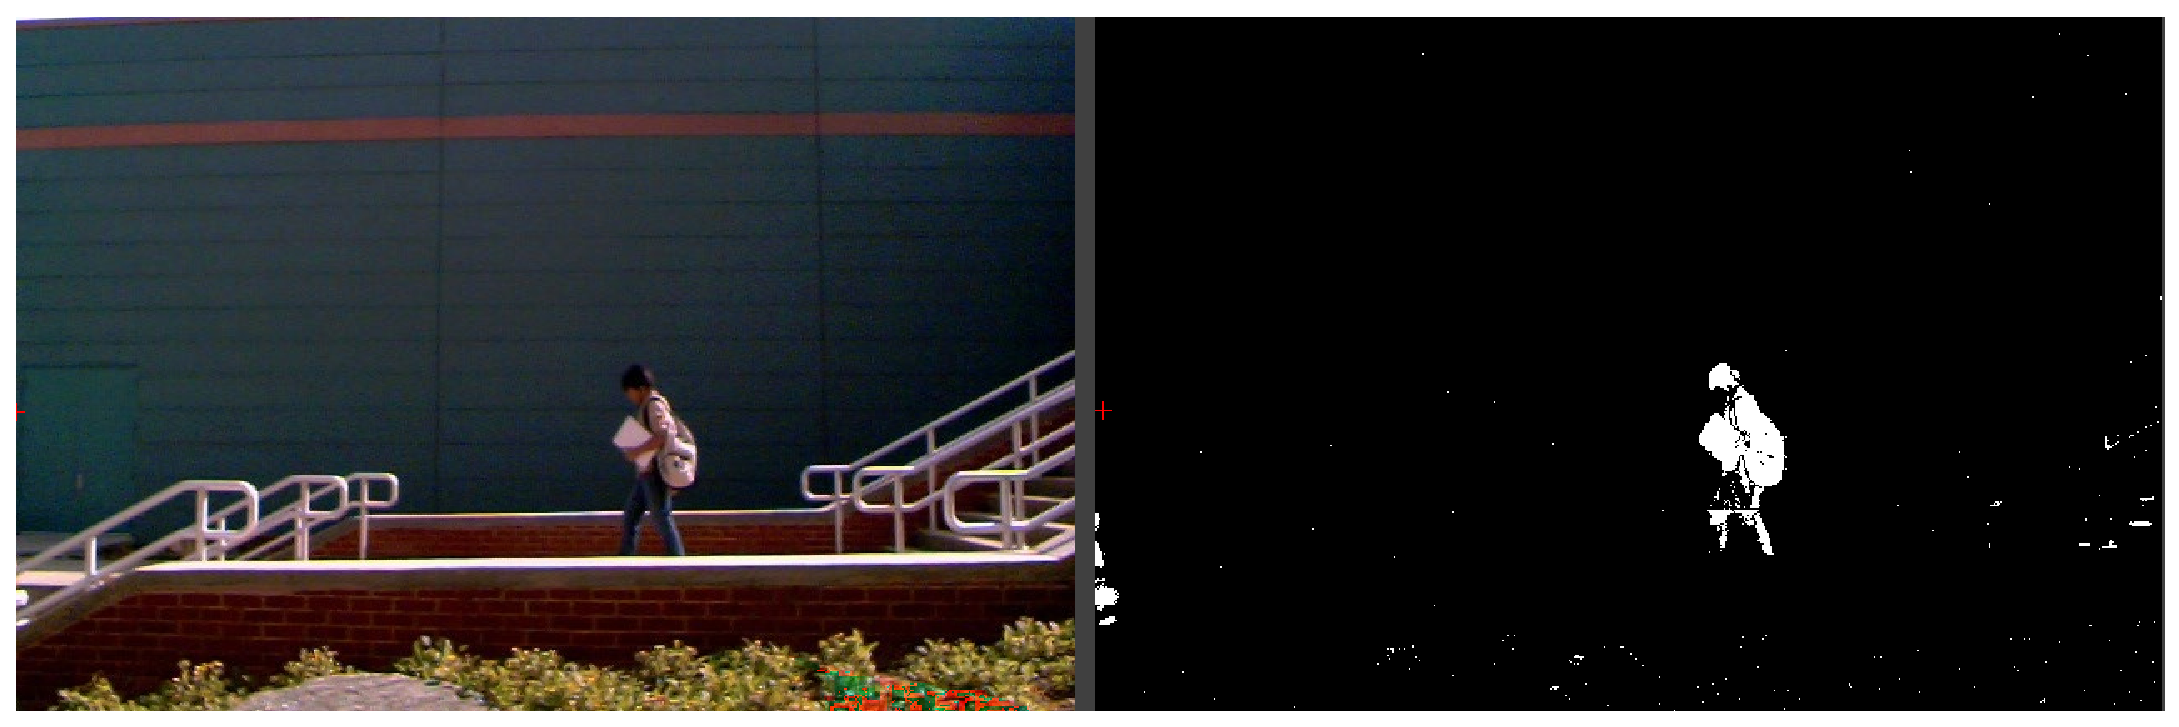
\includegraphics[width=1.0\textwidth]{figs/Proposal_fig12_TRK_multiGaussian}
					\caption{Multi-gaussian background subtraction.}
					\label{fig:MultiGaussian}
			\end{figure}
			
The Multi-gaussian algorithm for background modeling was introduced in \cite{1999_CNF_RealTimeTracking_Stauffer} and its use for target tracking was elaborated in \cite{2000_JNL_MG_Stauffer}.  In this algorithm, the background is modeled as a mixture of gaussians.  A decision is made as to which gaussians belong to the background, and which ones belong to the foreground.  This algorithm has already been explained in Section \ref{Sec:Origin}.  We implemented this algorithm on a PC and then ported it to a Texas Instruments TMS320DM642 Digital Signal Processor chip.  Certain time critical functions were coded in assembly to give up to 57x speed improvement.  However, the overall frame-rate remained at around 1 fps due to I/O bottlenecks.  While the porting of the algorithm to the DSP architecture did not directly impact the current research, it gave an appreciation of the issues involved in the pre-processing stages of tracking \cite{2008_TECH_MGDSP_Aslam}.  Moreover, the PC version of the algorithm serves as a pre-processing step of our currently implemented tracker.

			\begin{figure}		
					\centering		
					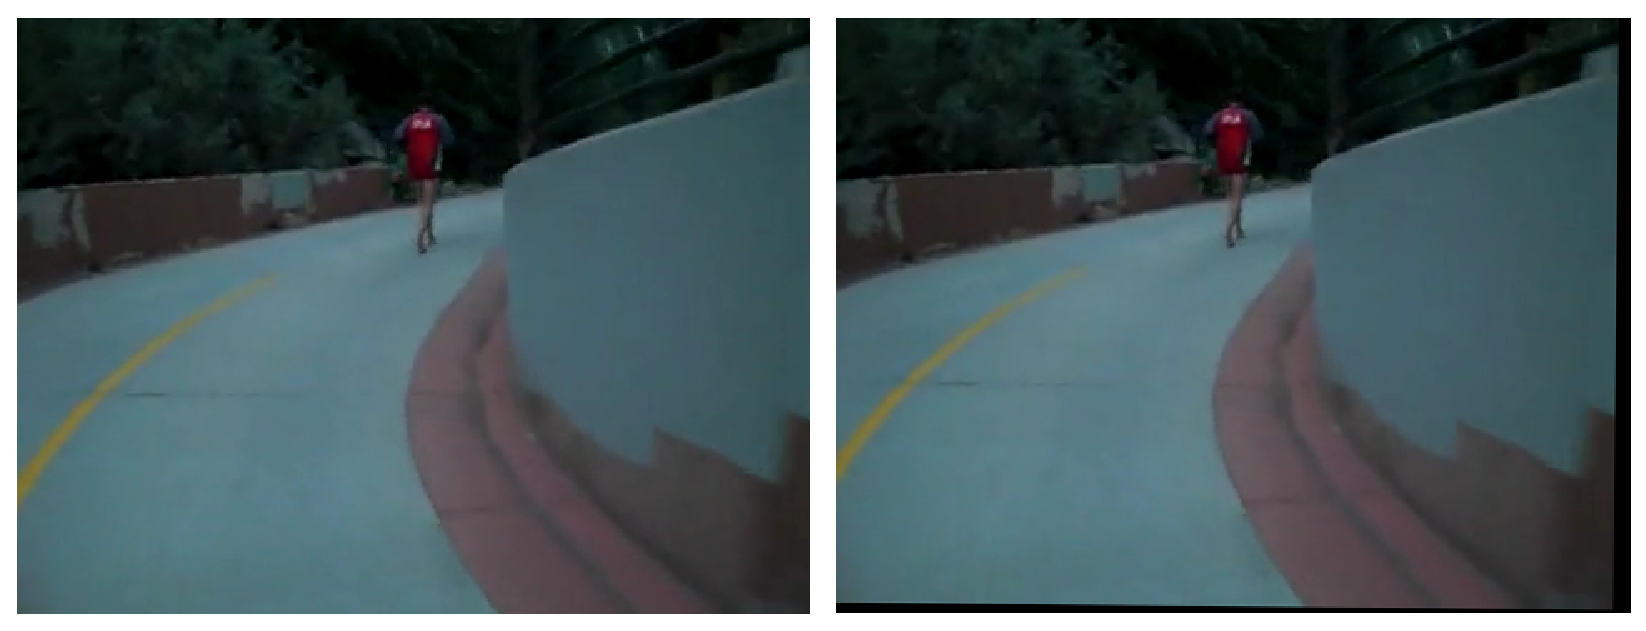
\includegraphics[width=1.0\textwidth]{figs/Proposal_fig13_TRK_deshaker}
					\caption{Video stabilization.}
					\label{fig:Deshaker}
			\end{figure}
			
\subsection{Pre-processing: Video Stabilization (patent applied)}
%===============================
Another pre-processing step that can be required if the video is shaky is video stabilization.  In particular, if a background modeling scheme is being used, then a shift of a few pixels can cause the entire model to fail.  Video stabilization allows alignment of successive images so that the background model can continue to update with registered pixel locations.  When a camera is shaking, camera shake motion vectors are superimposed on top of normal motion vectors, and normally have higher frequency.  Each motion vector is a sum of three components \cite{2006_CNF_Stabilization_Batur}:

\begin{equation}
\mathbf{V}_i(t) = \mathbf{O}_i(t) + \mathbf{P}(t) + \mathbf{J}(t)
\end{equation}  

Here, $\mathbf{O}_i(t)$ is the object motion at the $i$th scene location, $\mathbf{P}(t)$ is panning motion and $\mathbf{J}_(t)$ is the jitter motion.  Accumulated motion at each location of the image can be computed using a moving average filter.  Areas with lowest accumulated motion are then marked as areas to stabilize.  Once an area has been marked, its motion vectors are used to stabilize the whole image.  This algorithm was implemented on an Nvidia G92 GPU.  It ran at 55 frames per second on 1920x1080 HD \cite{2009_TECH_VideoStabilization_Arici}.  Figure \ref{fig:Deshaker} shows a snapshot of a shaky video and its stabilized version.  Although the effects of stabilization are difficult to appreciate on still images, the snapshot on the right shows black borders on the sides showing the extent of stabilization required for this particular image.

			\begin{figure}		
					\centering		
					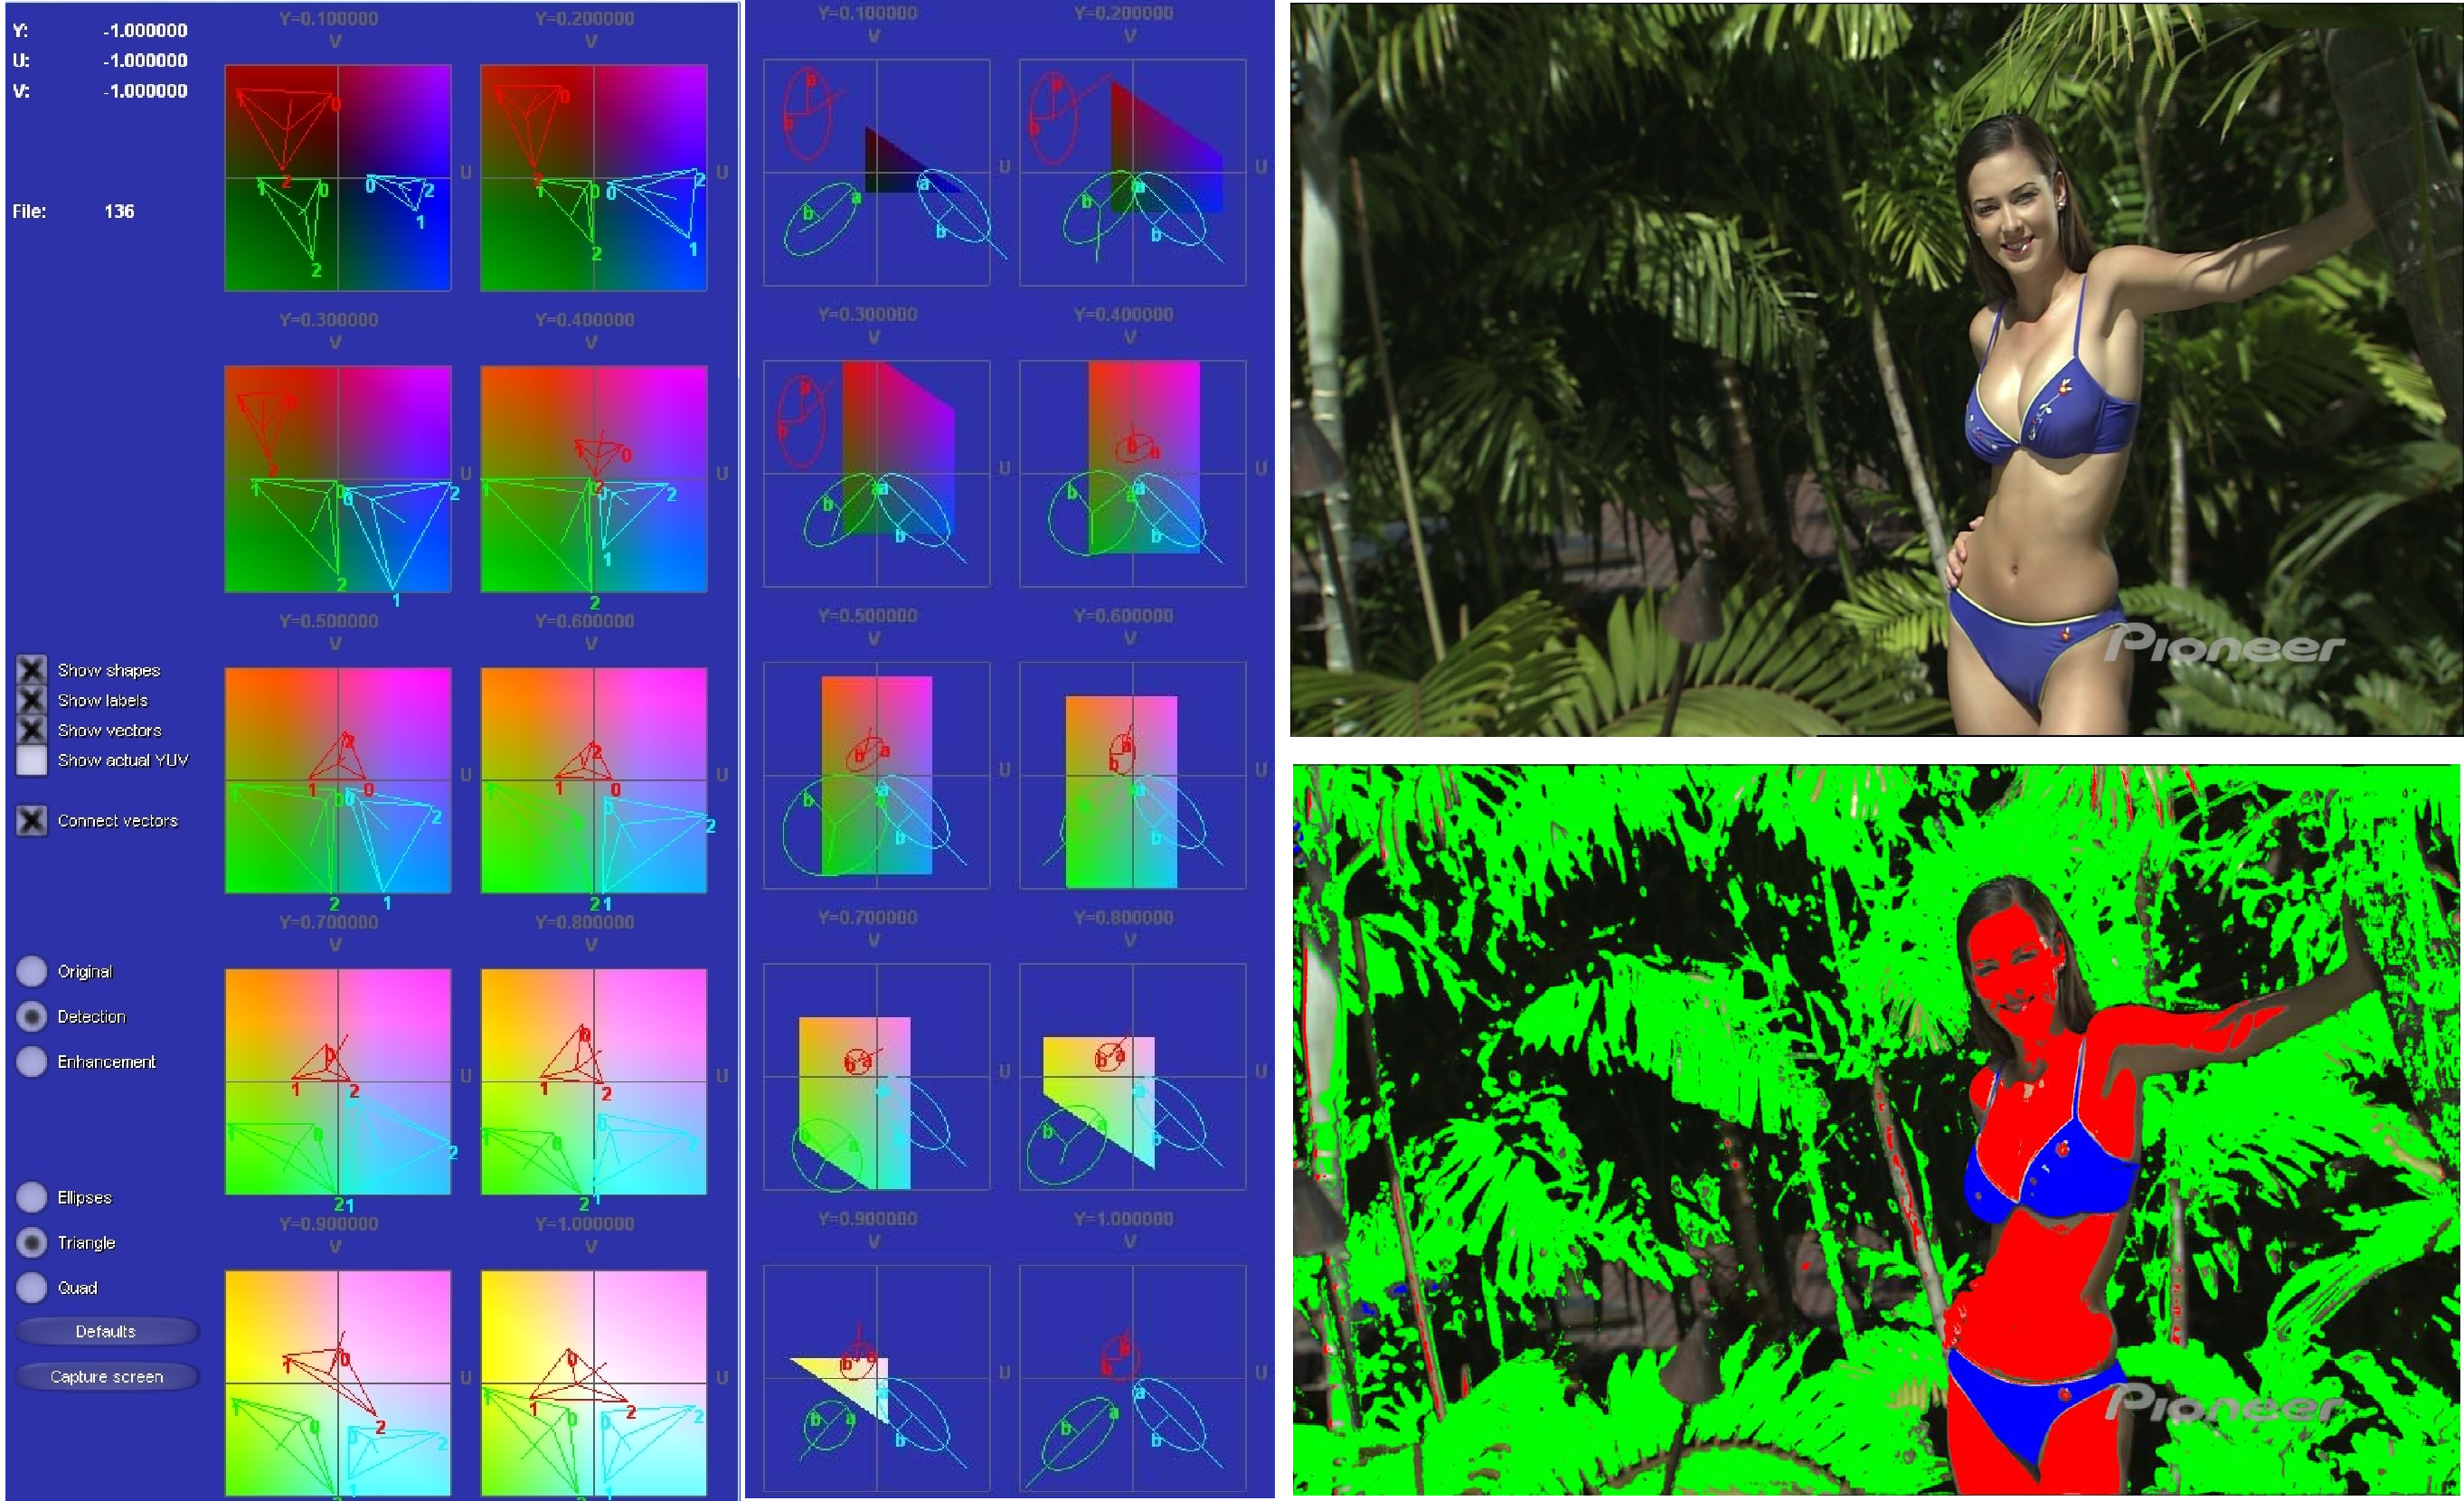
\includegraphics[width=1.0\textwidth]{figs/Proposal_fig14_TRK_colorDetection}
					\caption{Geometric figures in the YUV space to simultaneously detect multiple colors, including skin.}
					\label{fig:color_detection}
			\end{figure}
			
\subsection{Pre-processing: Feature Extraction (basis of patent)}
%==============================
Another aspect of target tracking is extracting features and tracking those features.  An important feature that has been widely used for tracking is color \cite{1997_CNF_ColorHeadTracking_Fieguth, 1998_CNF_HeadTracking_Birchfield, 2000_JNL_PersonTracking_Darrell, 2002_JNL_MeanShift_Comaniciu, 2002_CNF_TRKcolor_Perez}.  In this work, we develop a color detection technique in the 3D YUV color space \cite{2008_TECH_3DvideoColorEnhancement_Aslam}.  Triangles, quads or ellipses are placed at 10 quantized levels along the luma axis as shown in Figure \ref{fig:color_detection}.  During the training stage, the parameters of these geometric figures are adjusted to achieve optimum color detection.  During the testing phase, luma values are first quantized to one of the 10 pre-assigned levels.  This step is followed by a color detection step.  In practice, a linear interpolation of the geometric figures can be used, and is in fact the reason for using the linear YUV space rather than the non-linear HSV space.

			
			\begin{figure}		
					\centering		
					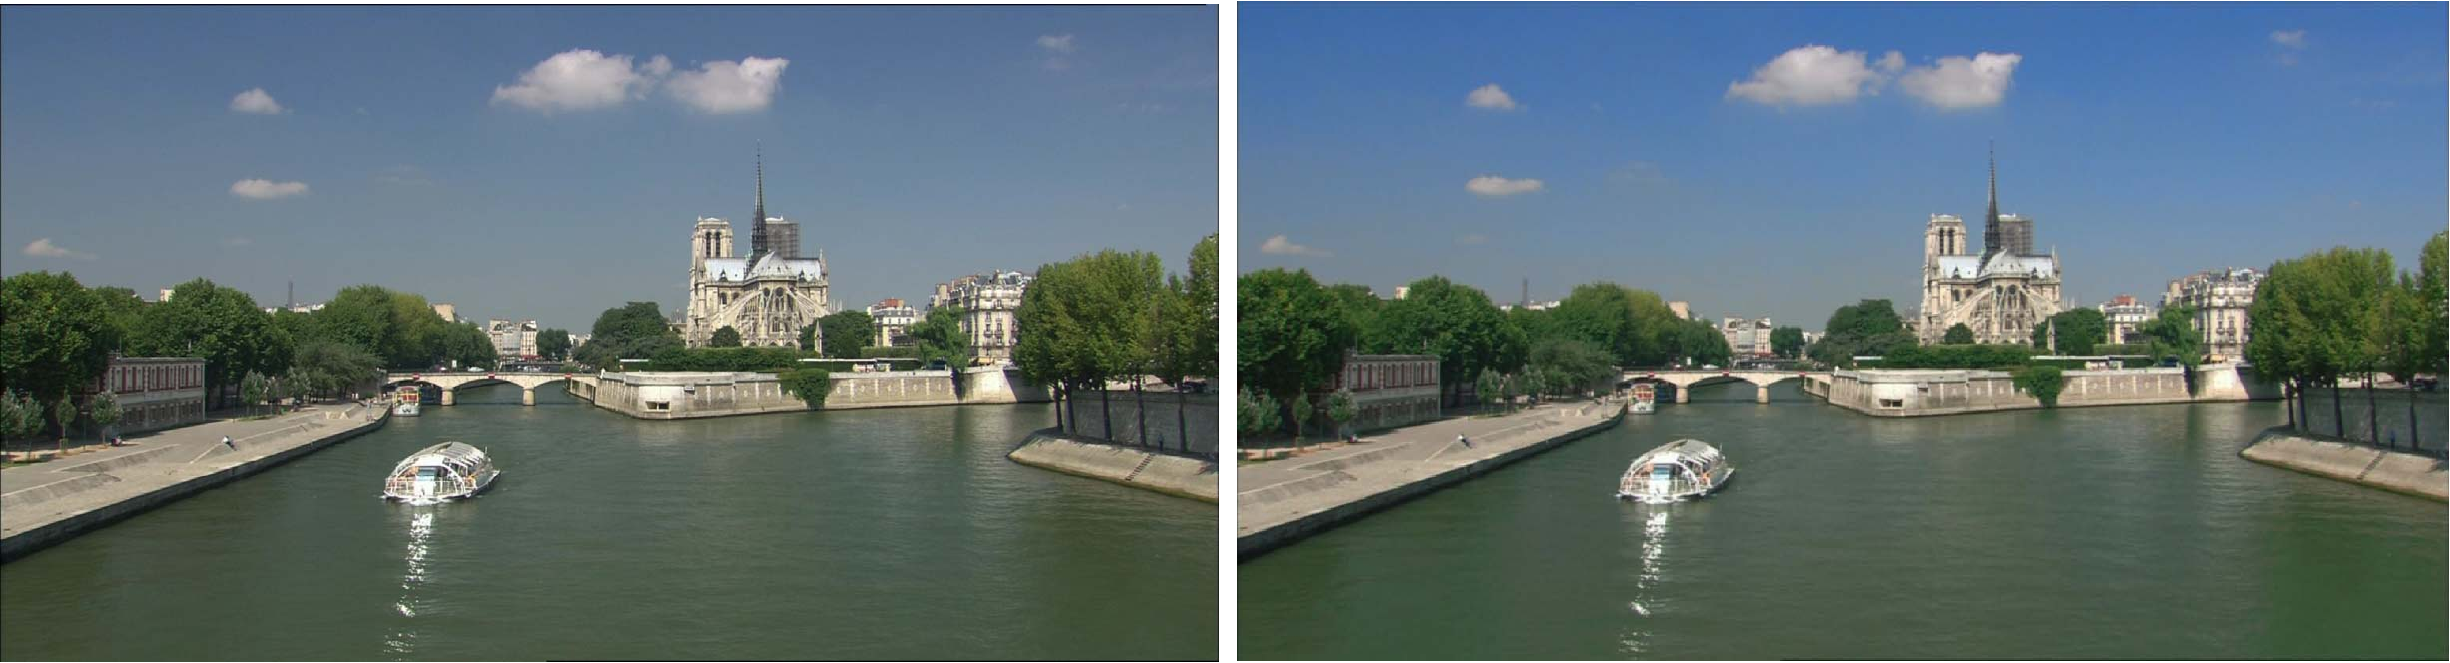
\includegraphics[width=1.0\textwidth]{figs/Proposal_fig15_TRK_colorEnhancement}
					\caption{Color enhancement}
					\label{fig:color_enhancement}
			\end{figure}

This software for color detection was created entirely in DirectX.  The detection operation was implemented using HLSL pixel shaders giving real-time performance on 1920x1080 HD video.  An additional feature of this software is color enhancement, as shown in Figure \ref{fig:color_enhancement}.

		\begin{figure}	
		\centering
		\subfigure[Geometric arrangement.]
		{
			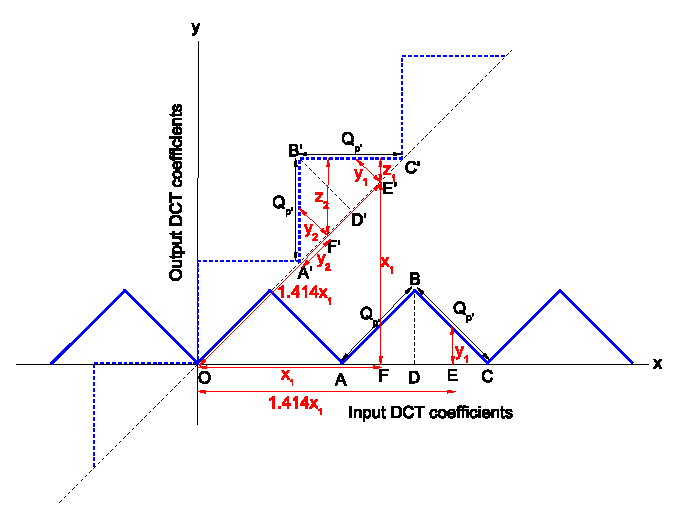
\includegraphics[width=0.47\textwidth]{figs/Proposal_fig16a_RVQ_MidriseQuantizerGeometry}
			\label{fig:MidriseQuantizerGeometry}
		}	
		\subfigure[Analytical equation plot.]
		{
			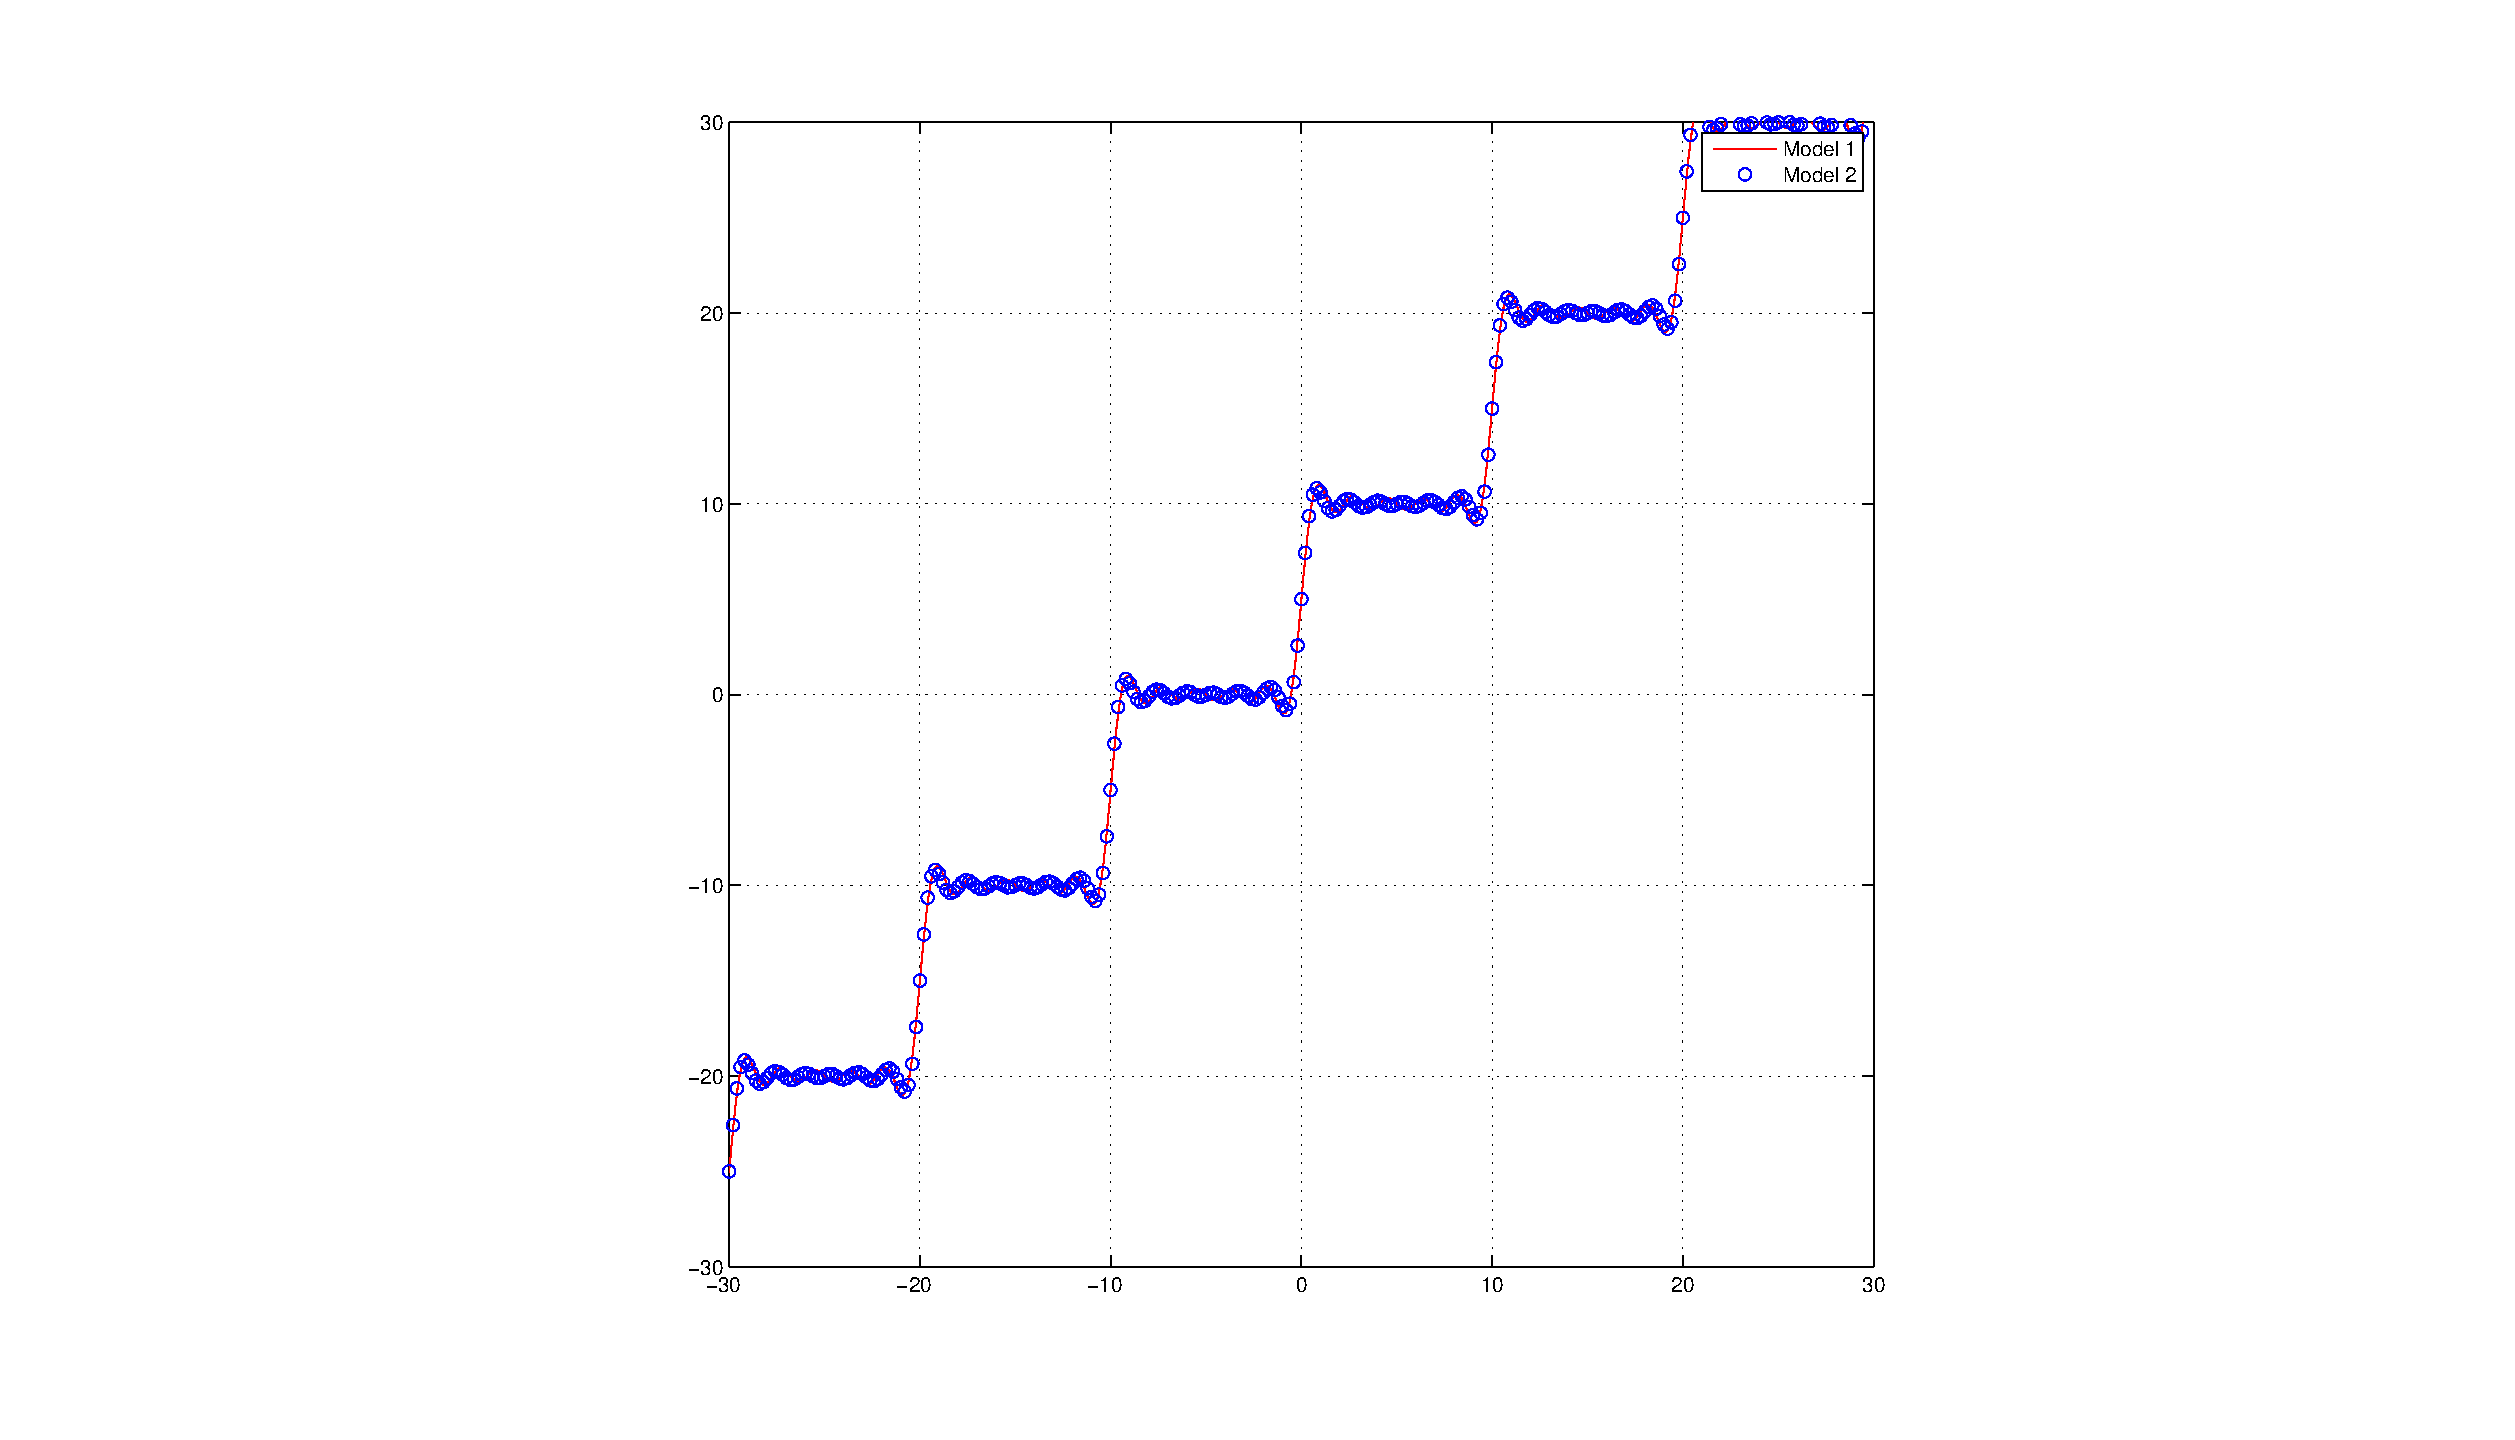
\includegraphics[width=0.47\textwidth]{figs/Proposal_fig16b_RVQ_MidriseQuantizerPlot}
			\label{fig:MidriseQuantizerPlot}
		}						
		\caption{Modeling the  midrise quantization function.}
		\label{fig:MidriseQuantizer} 	
		\end{figure}	
		
\subsection{Signal Compression: Modeling the Quantization Function}
%=============================================
After having mentioned the preliminary work on the main two thrusts of this research, tracking and RVQ, we now turn to the quantization function which is the basis of any compression system, such as RVQ.  In \cite{2010_CNF_Quant_Aslam}, we try to find an analytical function for a mid-rise quantizer.  Although this problem has been studied in detail, our goal is to understand the dependence of the quantizer waveform on the quantization parameter.  Through an alternate geometric arrangement shown in Figure \ref{fig:MidriseQuantizerGeometry}, we model this function as a sequence of two fourier series.  Effectively, the equation comes out to be


		\begin{align}
		z[x] &= DC + 2 \ c_{s_2}[1] \ cos( w_0 \ x) + 2 \ c_{s_2}[3] \ cos(3 \ w_0 \ x) + 2 \ c_{s_2}[5] \ cos(5 \ w_0 \ x)\notag\\
		 			 &= DC + 2 \ c_{s_2}[1] \ cos( \frac{2 \ \pi}{Qp\,^{\prime}}x) + 2 \ c_{s_2}[3] \ cos(3 \ \frac{2  \  \pi}{Qp\,^{\prime}}x) + 2 \ c_{s_2}[5] \ cos(5 \ \frac{2  \ \pi}{Qp\,^{\prime}}x)
		\label{eq:Square_2_time}
		\end{align}
			
Here $c_{s_2}$ are the coefficients of yet another Fourier Series.  The output of this function is plotted in Figure 	\ref{fig:MidriseQuantizerPlot}.  It is clear that it closely models the mid-riser quantizer function.			

%##############################################################################################################
\newpage
\section{Proposed Research}
\label{proposed}
%##############################################################################################################
\subsection{Expected Title}
The title of the Ph.D. dissertation is expected to be \emph{Multi-Target Tracking Using Residual Vector Quantization}.

\subsection{Abstract}
The objective of the proposed research is to track multiple targets in an image sequence using Residual Vector Quantization and under conditions of target to target occlusions. 

Multi-target visual tracking is an important problem.  It is also a challenging problem.  However, if there are no occlusions, i.e. no missed observations, the problem becomes one of state estimation that can be handled by standard tracking methods \cite{1972_CNF_PDAF_BarShalom,1975_JNL_PDAF_BarShalom,1978_JNL_SURVEYmtt_Barshalom,1983_JNL_JPDAF_Fortmann,2009_JNL_PDAF_Barshalom, 1997_CNF_UKF_Julier, 1998_JNL_Condensation_IsardBlake}.  Our goal therefore is to try and solve the multi-target problem under occlusions.  There are two basic kinds of occlusions (a) Target to target occlusions, in which it is assumed that only targets that are being tracked will occlude each other, (b) Background to target occlusions, in which it is assumed that background objects can occlude targets.  In this work, we limit ourselves to target to target occlusions.  So far, we have experimented with RVQ on a small scale multi-target tracking problem and found encouraging results \cite{2010_CNF_TrkRVQ_Aslam}.  To get a better feel for how RVQ behaves, we have also experimented with using it to recognize human action in conjunction with an HMM \cite{2010_CNF_TrkRVQ_Aslam}.  Prior to this experimentation with RVQ, we have worked with background modeling \cite{2008_TECH_MGDSP_Aslam}, color feature extraction \cite{2008_TECH_3DvideoColorEnhancement_Aslam}, video stabilization, tracking on low bit rate video \cite{2009_CNF_CVcompMS1_Aslam,2009_CNF_Compensation_Aslam}, contour tracking \cite{2010_CNF_VehicleContour_Aslam}, and modeling the midrise quantizer function \cite{2010_CNF_Quant_Aslam}.  All these are components of a tracker based on a Residual Vector Quantizer.  In the future, we believe that this preliminary investigation, along with the following five step approach, will advance the solution of the problem at hand: (a) gather training data, (b) choose RVQ design mode (c) information fusion, (d) optimizing RVQ detection performance, and (e) time evolution of RVQ codebooks.  We elaborate on these steps in the following paragraphs.


%##############################################################################################################
\newpage
\section{Work remaining to be done}
\label{remains}
%##############################################################################################################

As described in Section \ref{Sec:Preliminary}, our work \cite{2010_CNF_TrkRVQ_Aslam, 2010_CNF_HMMRVQ_Aslam} is the first reported use of RVQ for any form of video analysis.  In \cite{2010_CNF_TrkRVQ_Aslam} we have used RVQ as an unsupervised detection system in a multi-target tracking system \cite{2010_CNF_TrkRVQ_Aslam}.  This approach is similar to the unsupervised classification approach used by \cite{1998_CNF_Tracking_Lipton}.  Initial results were promising as RVQ was able to differentiate between targets using limited training samples in a high dimensional data space.  Other researchers have used an offline training stage to train the classifier on training samples drawn from a distribution similar to the distribution from which the test samples will be drawn.  For example, a supervised SVM based classification method was used effectively in \cite{2004_JNL_SVMtracking_Avidan} to detect and track cars.  This approach of augmenting the tracker with a trained classifier holds promise.  Since RVQ has been demonstrated to act as a classifier \cite{2007_JNL_IDDM_Barnes}, our goal is to use RVQ as a detector/classifier that aids in the task of target correspondence, and therefore we anticipate results in more robust tracking.  

Given the fact that we would like to use RVQ in a classifier/detector role in the multi-target tracking scenario, we envision our future work evolving according to the general steps given below. 

\subsection{Step 1. Gather training data}
%================================
Gather sufficient training data that can generate a representative distribution of the test data.  

\subsection{Step 2. Choose training mode}
%================================
RVQ training can be done in two ways: (a) Training on entire targets, as in \cite{2010_CNF_HMMRVQ_Aslam, 2010_CNF_TrkRVQ_Aslam}, and  (b) Training on components of the target.  For non-rigid targets, such as humans, the latter approach may be more appropriate since the overall shape and appearance can change quite dramatically from frame to frame.  Moreover, as some parts of the target get occluded, other parts may still be visible giving us some positive detections.  However, this would require an additional step of fusing information from the various component detections.  Another aspect to keep in mind here is that the RVQ codebooks encode visual aspects of objects such as appearance and shape.

\subsection{Step 3. Fuse information from various detections}   
%================================
This is the heart of the inference system that we intend to build.  For action detection, we used an HMM \cite{2010_CNF_HMMRVQ_Aslam} as the inference engine.  For multiple detections returned per target, we need a way to fuse the information to give us a probabilistic measure of assigning a label to a target.  Moreover, other computed features, such as corners can also be input into the inference system.  A Dynamic Bayesian network (DBN) such as an HMM may not be appropriate for individuals in a dense crowd since it would be difficult to compute transitions between states over time and to update the models with time.  Another kind of DBN, such as particle filters, that incorporate a dynamical system, along with state transition probabilities, may be more useful for correspondence and inference over time.  At a given time instant though, on the spatial level, an undirected graphical model may be appropriate to reconcile all the feature and detection labels generated in a specific neighborhood.  Markov Random Fields (MRFs) are a kind of undirected graphical model that provide a natural way of penalizing solutions that are inconsistent with the observed data and with smoothness priors.  Pixel-labeling problems are naturally represented in terms of energy minimization which can be justified in terms of MAP estimation in MRFs \cite{1984_JNL_StochasticRelaxation_Geman, 2008_JNL_MRF_Szeliski}, and since RVQ returns per pixel detections, this framework could lend itself naturally to a spatial inference system feeding from an RVQ classifier.  Conversely, we could also model causal relationships in the spatial domain using a directed static Bayesian network.  Using one of these inference engines, our goal would be to assign correct labels to our targets as they merge, split, and emerge from occlusions.  We make the assumption that only target to target occlusions occur, and no target is occluded by the background.

\subsection{Step 4. Optimizing detection performance from RVQ} 
%================================
The RVQ engine will return different information depending on the number of code-vectors per stage and number of stages.  Together, these two parameters define an encoder/decoder pair.  During the testing phase, the stage depth is another parameter that will affect RVQ output.  A few code-vectors per stage will have higher generalization ability but will provide more crude approximations to the source symbols.  

\subsection{Step 5. Time evolution of the codebooks} 
%================================
The final envisaged step is the time evolution of the codebooks.  The reason is that appearance models change over time.  In the very least, there is a steady drift.  Moreover, as targets deform, their appearance models can change drastically.  If the code-vectors are not updated with time, the joint distribution over the source symbols and RVQ code-vectors that were generated during training will no longer match the test data, and the classifier will increasingly perform poorly.  \cite{1998_CNF_Tracking_Lipton} handle this problem by updating their templates using an IIR filter.  In our case, it is expected that the code-vectors at the initial stages will drift more slowly than the code-vectors in the later residual stages.

It is expected that if implemented well, the above mentioned steps should provide a direction towards the solving of the occlusion problem in multi-target visual tracking.  It may be noted that we will carry out our experiments with a static camera so as to eliminate a large source of error.  Only if the occlusion problem is solved should this work be extended to the moving camera case.  Also, for the sake of completeness, we mention that multi camera systems can in many ways alleviate the occlusion problem.  Nevertheless, multiple cameras are not always available, synchronization is normally problematic, correspondence can be cumbersome and so it is desirable to solve the problem at hand with one camera, and then to proceed to multiple cameras.


%##############################################################################################################
\newpage
\section{Facilities and Equipment Needed}
\label{facilities}
%##############################################################################################################

\subsection{Hardware}

The following hardware is needed for further experimentation in the proposed area of research:

\begin{enumerate}
\item \textbf{Laptop}: Implement algorithms and process images and videos captured with visual sensors.

\item \textbf{Video Camera}: Record motion sequences that are tailored to our exact needs. 

\item \textbf{Still Camera}: Record still shots of subjects at high resolution.  

\item \textbf{Tripod}:  Our experiments will be with a camera that is not shaking.  A tripod is necessary to guarantee that.
\end{enumerate}

\subsection{Software}
The following software is also required:

\begin{enumerate}
\item \textbf{Matlab}: Matlab is a general purpose scripted computing environment. 
\item \textbf{C compiler}:  A C compiler is required to compile time critical C language modules.  Microsoft Visual Studio is the preferred choice due to its extensive .NET library.
\item \textbf{Libraries}: Various libraries will be used including Intel OpenCV and OpenGL.
\end{enumerate}











%##############################################################################################################
\end{Body}
\begin{EndMatter}
\references% Generates the bibliography page
\end{EndMatter}
\end{document}

%##############################################################################################################
%##############################################################################################################

%\begin{enumerate}
%\item \textbf{2-D approach without explicit shape models}.  In \emph{grid based methods}, a grid is imposed on the region of interest and features computed in tiles of the grid may be combined to form a feature vector, for instance, sum of normal flow \cite{1994_CNF_GetYourMan_Polana} or number of foreground pixels \cite{1992_CNF_HumanActionHMM_Yamato}.  In \cite{1998_JNL_AutonomousDriving_Franke}, PCA is applied on a grid representation of blurry pedestrian silhouettes.  Grid-based methods make it relatively straightforward to deal with partial occlusions \cite{1999_JNL_SURVEYmotion_Gavrila}. \emph{Classifier based methods}.  \cite{1997_CNF_PedestrianDetection_Oren} train an SVM classifier on wavelet coefficients trained on regions of interest.  This classifier is then used to detect pedestrians.
%
%\item \textbf{2-D approach with explicit shape models}.
%\end{enumerate}
%
%Johansson showed that we can directly use motion for action recognition \cite{1973_JNL_VisualPerception_Johansson}.  There are 2 theories about this interpretation: (1) People use motion information to recover 3-D structure (structure from motion) and use this structure for activity recognition (2) People use motion information for direct \emph{motion-based} recognition.  Our approach is related to the latter.  There are 2 further steps in this approach: (a) An appropriate representation of the object/motion (b) Matching an unknown input with some form of model \cite{1995_JNL_SURVEYmotion_Cedras}.

%Another approach is to combine classification with tracking.  \cite{2004_JNL_SVMtracking_Avidan} tracks cars using a Support Vector Machine \cite{1992_CNF_TrgOptimalMarginClassifiers_Boser} classifier for detection.  A local SVM score is maximized in combination with satisfying optical flow constraints to track vehicles.
%The pixel process is not stationary.  Therefore, one cannot resort to maximizing the likelihood of the observed data using the Expectation Maximization (EM) algorithm.  